\section{Numerical Results and Comparisons}\label{sec:results}


The solutions to the PNP problem exhibit a specific behavior that was 
described above. In order to find the best adaptive method to deal with 
this type of problems, we performed numerous computations using all 
adaptivity modes in both the single-mesh and multi-mesh regimes.
In the numerical experiments we paid attention to the 
relative error, cumulative CPU time, and problem size 
in terms of number of degrees of freedom (DOF) in each 
time step. 

We used two types of initial meshes --- a finer mesh shown 
in Fig.~\ref{fig:mesh}~(c) was used for \emph{p}-adaptivity
and a very coarse initial mesh shown in  Fig.~\ref{fig:mesh}~(a) was 
used for $h$-adaptivity and $hp$-adaptivity.

\begin{figure}[!ht]
  \begin{centering}
  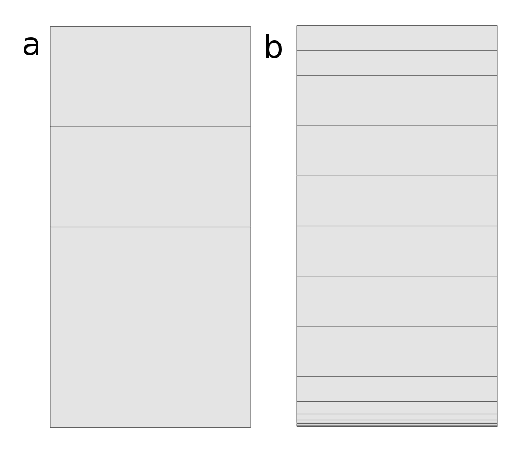
\includegraphics[width=.8\columnwidth]{mesh}
  \caption{\label{fig:mesh} Initial coarse mesh (a),
  	half refined mesh (b) and refined mesh (c). The coarse mesh (a)
	and refined mesh (c) were used in the initial calculations, the latter one
	in case of \emph{p}-adaptivity (including HP\_ANISO\_P). The half-refined mesh (b) was
	used later to optimize the \emph{hp}-adaptive refinement solutions.}
  \end{centering}
\end{figure}

An example of the solution at $t=0.7\ s$ and $t=3.0\ s$ 
calculated with the HP\_ANISO refinement mode is shown
in Figs.~\ref{fig:cphi-1} and \ref{fig:cphi-2}. 

\begin{figure}[!ht]
  \begin{centering}
  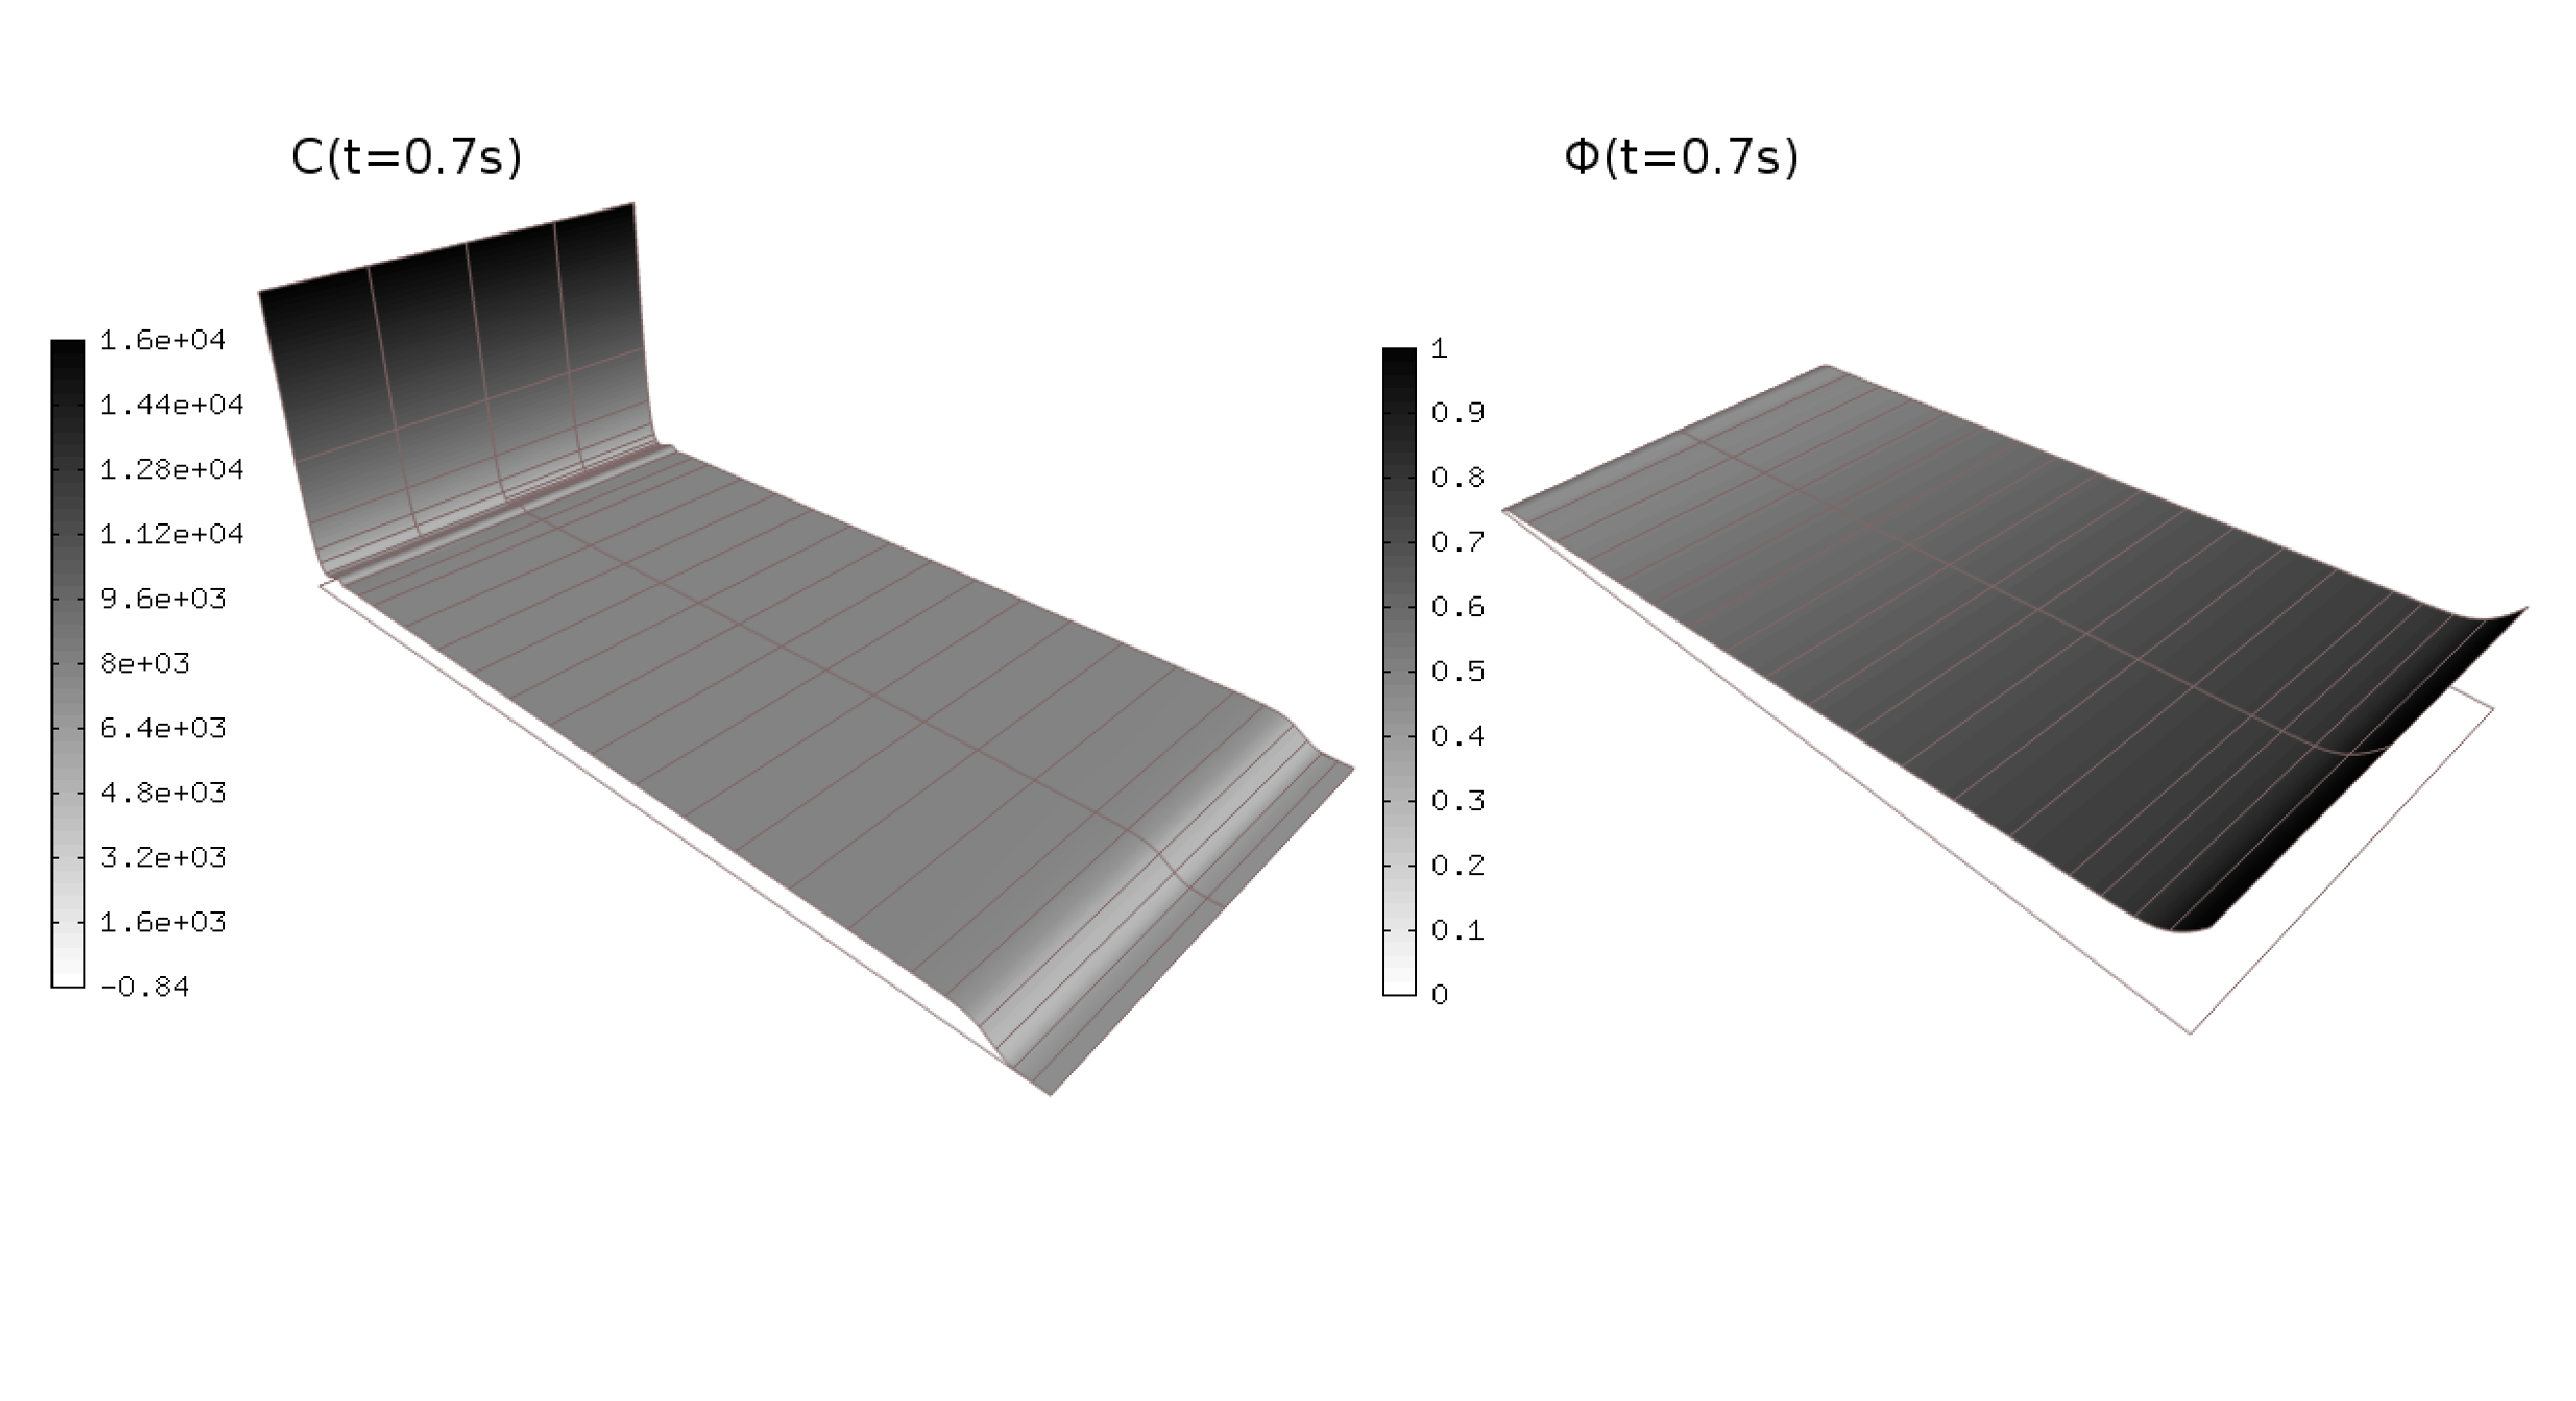
\includegraphics[width=.75\columnwidth]{cphi-1}
  \caption{\label{fig:cphi-1} Concentration $C$
  and voltage $\phi$ at $t=0.7\ s$.}
  \end{centering}
\end{figure}

\newpage

\begin{figure}[!ht]
  \begin{centering}
  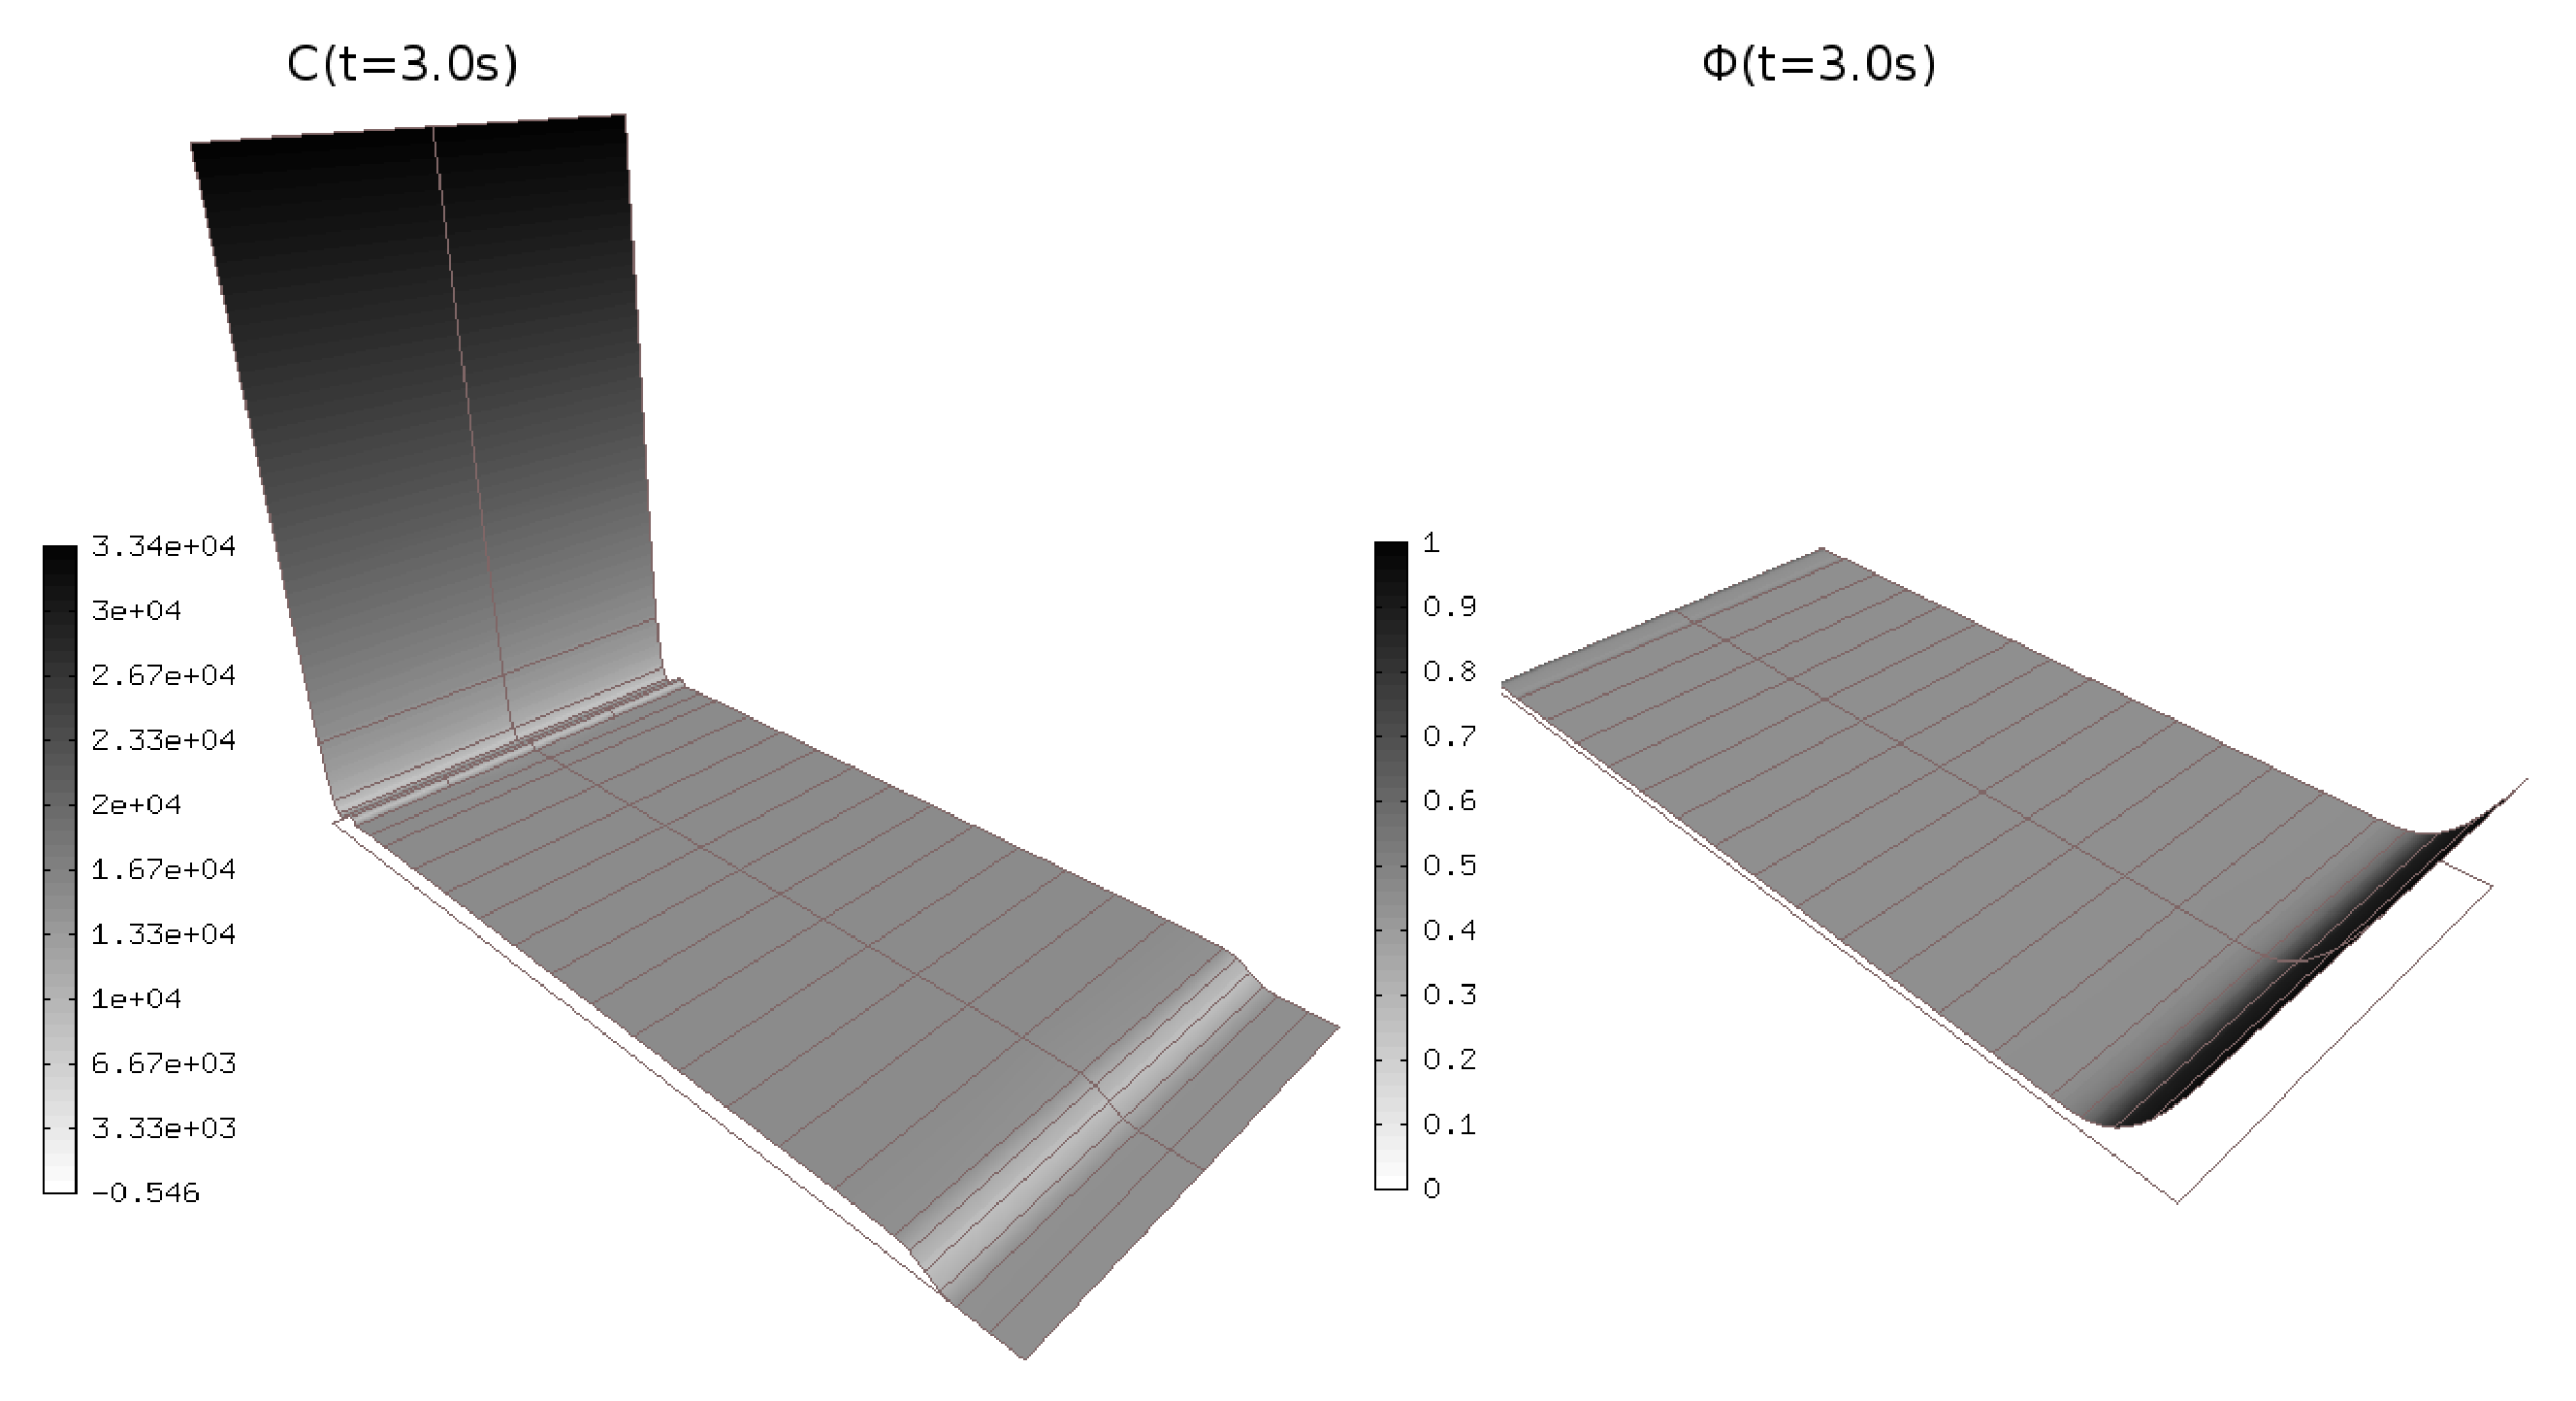
\includegraphics[width=.75\columnwidth]{cphi-2}
  \caption{\label{fig:cphi-2} Concentration $C$
  and voltage $\phi$ at $t=3.0\ s$.}
  \end{centering}
\end{figure}

The reader can see that at $t=0.7\ s$ some ionic migration has already 
taken place and large concentration gradients near the boundaries $\partial\Omega_1$ 
and $\partial\Omega_3$ have formed. The figures also show that the meshes 
at $t=0.7\ s$ and $t=3.0\ s$ are different. 

\subsection{Comparison of single mesh low-order FEM and $hp$-FEM}

Comparison of single mesh H\_ANISO with p=1, single mesh H\_ANISO with p=2
and single mesh HP\_ANISO should be added here to make the point that 
hp-FEM is much better than low-order FEM. 
Otherwise the reader does not know 
why we are just using hp-FEM in the following. Or is there a reason 
why you do not want to add this here --  long computing time for hp-FEM or something 
else?

\subsection{Comparison of single-mesh and multi-mesh $hp$-FEM}

Running the simulation with different adaptivity modes 
and meshes showed that the multi-mesh $hp$-FEM configuration resulted into
the smallest problems, shortest computing times, and better or the same error 
convergence compared to any single-mesh configuration.
This is illustrated in Figs.~\ref{fig:singlemultidof} 
and Fig.~\ref{fig:singlemulticpu}.

\begin{figure}[!ht]
  \begin{centering}
  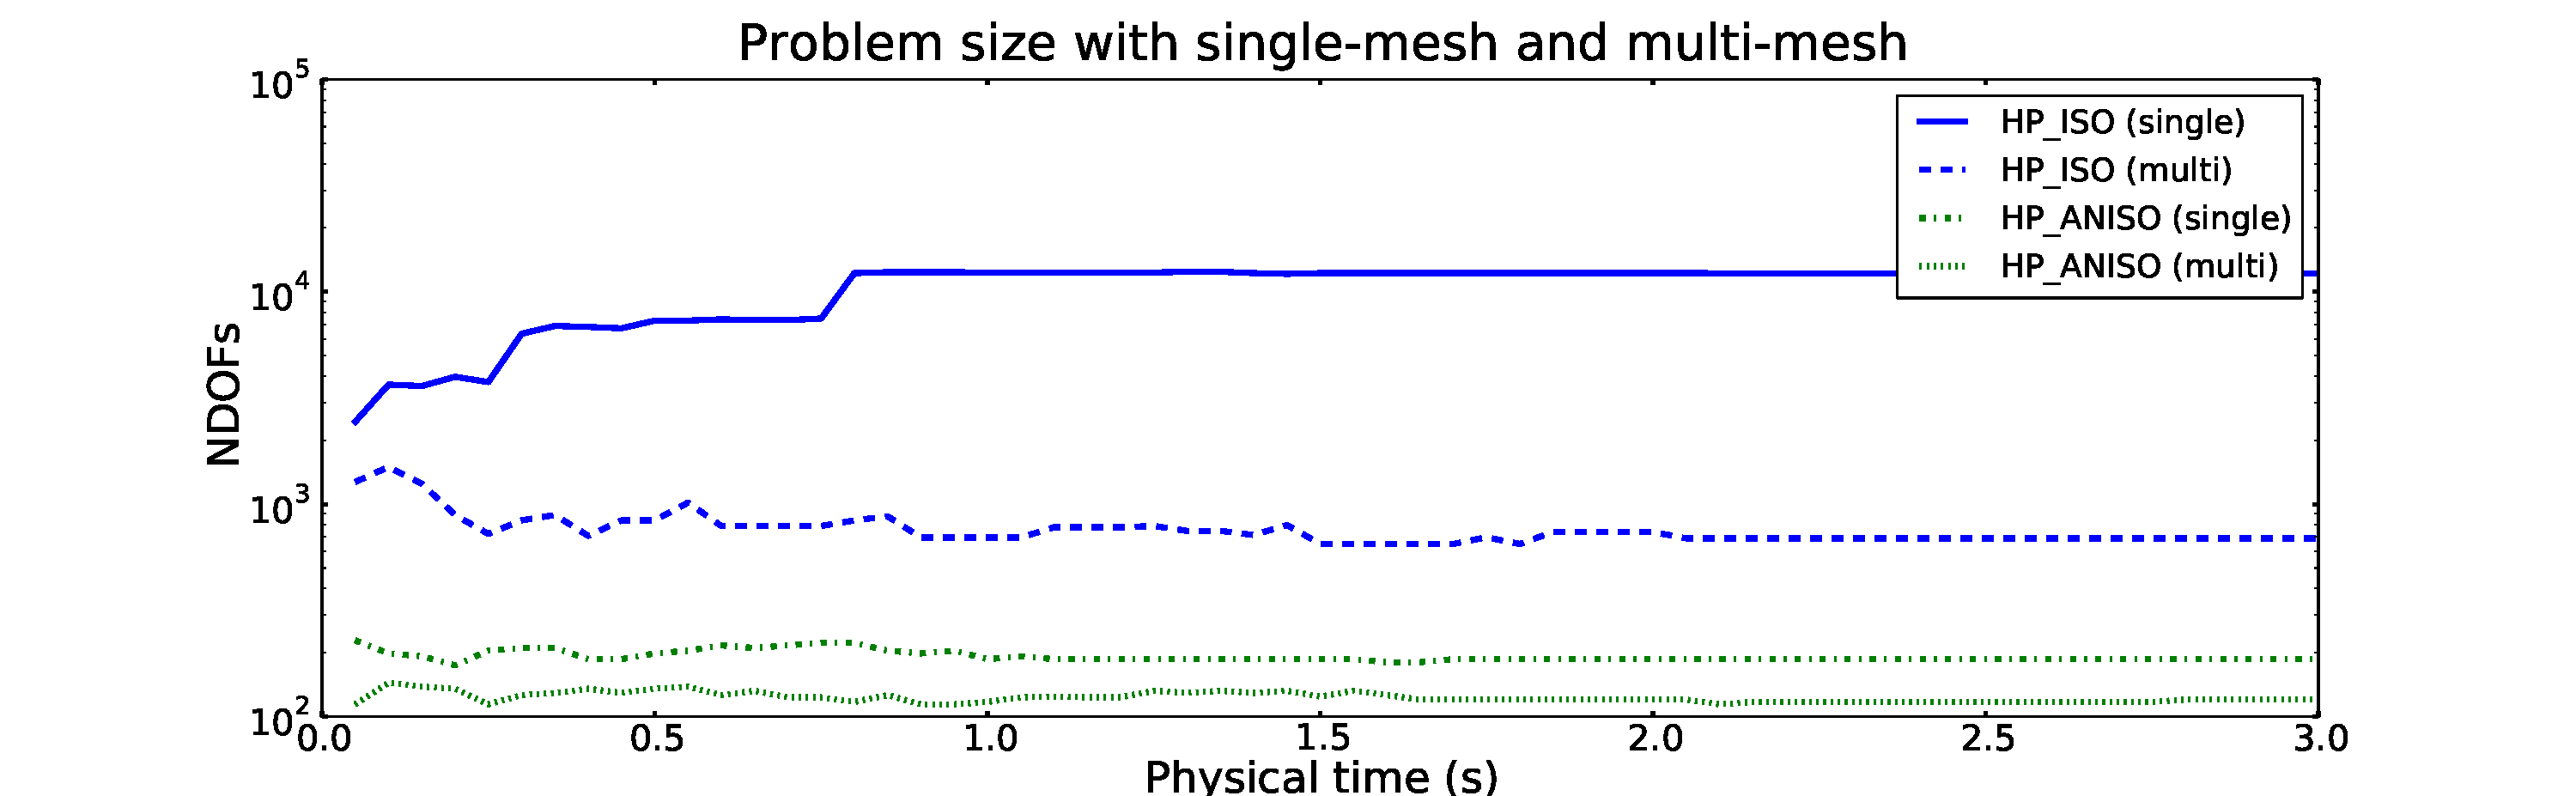
\includegraphics[width=\columnwidth]{singlemulti_dof}
  \caption{\label{fig:singlemultidof} Number of degrees of freedom (DOF) as a function 
  of physical time for single-mesh and multi-mesh configurations with the HP\_ISO
  and HP\_ANISO adaptivity modes. Note logarithmic scale on the vertical axis.}
\vspace{-6mm}
  \end{centering}
\end{figure}


\begin{figure}[!ht]
  \begin{centering}
  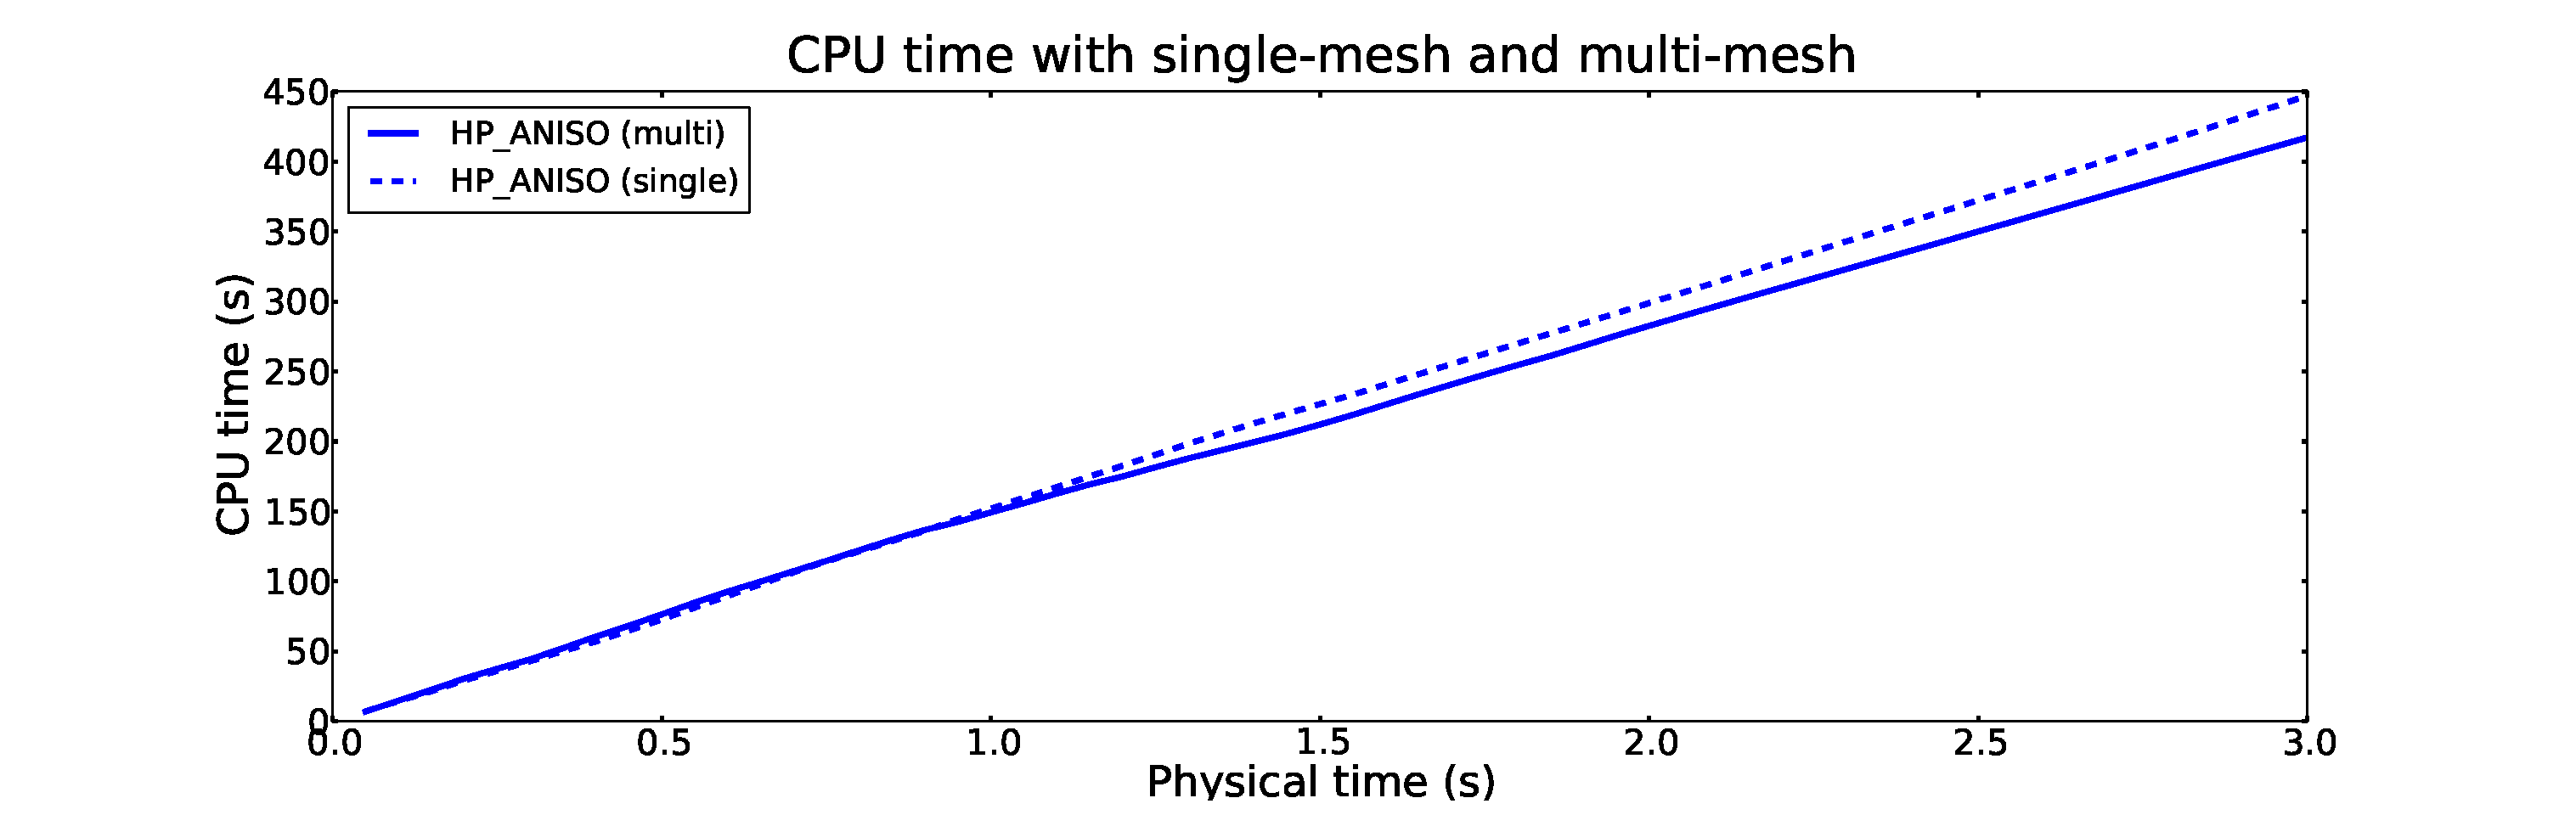
\includegraphics[width=\columnwidth]{singlemulti_cpu}
  \caption{\label{fig:singlemulticpu} Cumulative CPU time as a function 
  of physical time for single-mesh and multi-mesh configurations with the HP\_ISO
  and HP\_ANISO adaptivity modes. Note logarithmic scale on the vertical axis.}
  \end{centering}
\end{figure}

\noindent 
Fig. \ref{fig:poly} shows higher-order meshes in the adaptive multimesh $hp$-FEM
computation for $C$ and $\phi$ at $t = 0.7$ s. Different 
colors mean different polynomial degrees. A diagonal pattern inside an element 
tells that the element has different polynomial degrees in the 
horizontal and vertical directions. 


\begin{figure}[!ht]
  \begin{centering}
  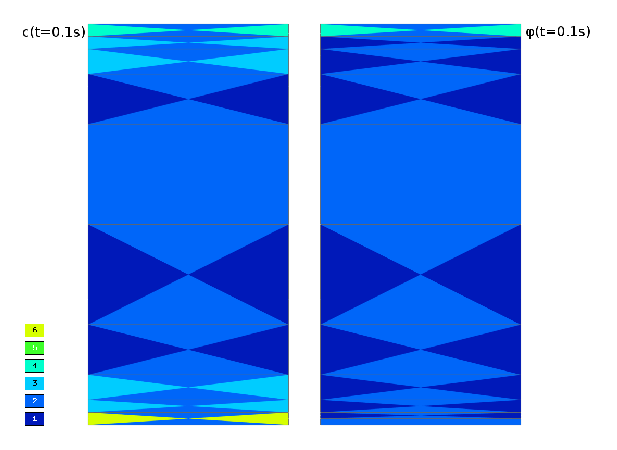
\includegraphics[width=.75\columnwidth]{poly}
  \caption{\label{fig:poly} Higher-order FEM mesh for 
  $C$ and $\phi$ at $t=0.7\ s$. }
  \end{centering}
\end{figure}

These result are in good agreement with Fig.~\ref{fig:cphi-2} -- in the vicinity
of the boundaries $\partial \Omega_1$ and $\partial\Omega_3$, the concentration gradient
is much greater than the voltage gradient. Therefore the multimesh $hp$-FEM adaptivity 
algorithm has increased the maximum polynomial degree for the $C$-space to~7 while 
the maximum polynomial degree for the $\phi$-space is~2. One can also see that the mesh 
is significantly more refined for $C$.
Since these results are representative for all adaptivity modes, only multi-mesh 
configurations are considered in the following. 

\subsection{Comparison of isotropic and anisotropic refinements}

Next we would like to illustrate the role of anisotropic mesh refinements.
Figs.~\ref{fig:isoanisodof} and \ref{fig:isoanisocpu} show typical results 
for the H\_ISO, H\_ANISO, HP\_ISO, HP\_ANISO adaptivity modes in terms 
of DOF and cumulative CPU time.


\begin{figure}[!ht]
  \begin{centering}
  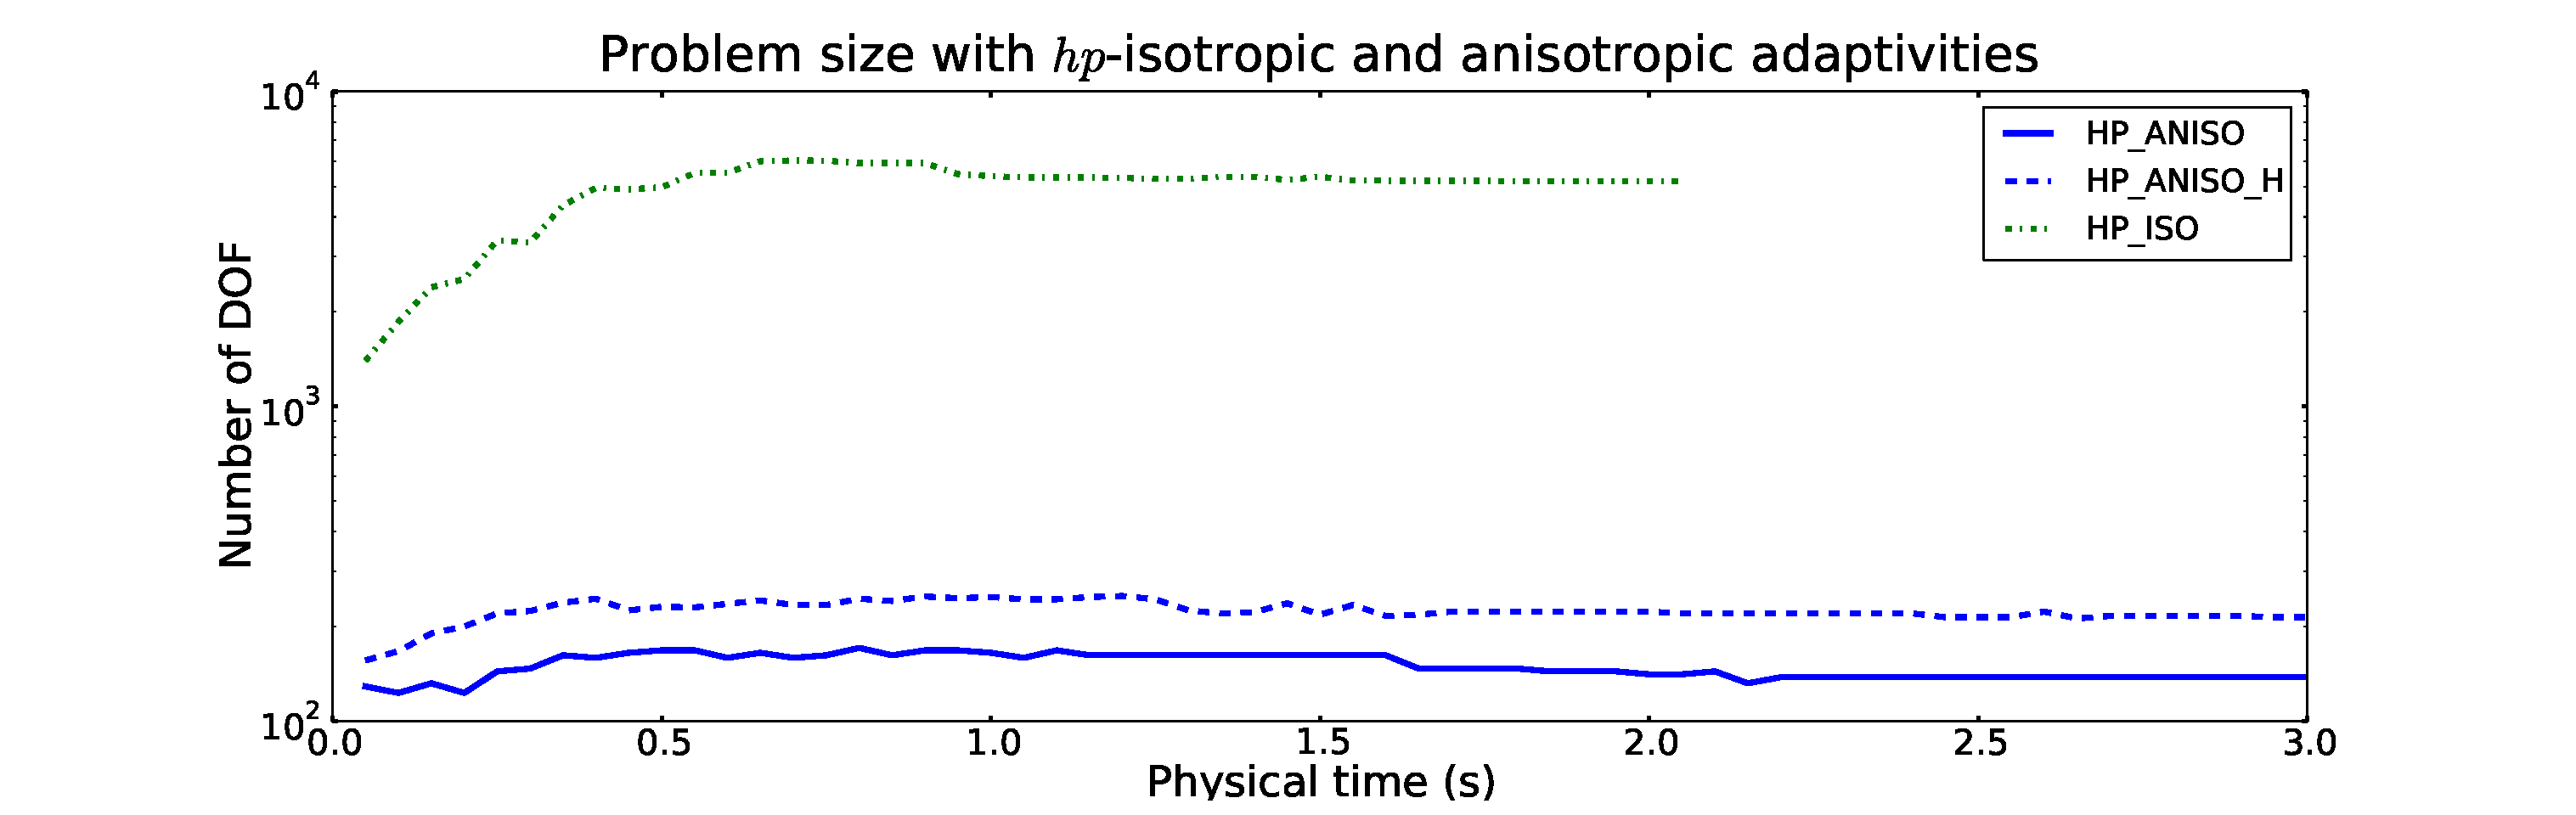
\includegraphics[width=\columnwidth]{isoaniso_dof}
  \caption{\label{fig:isoanisodof} Number of DOF as a function of physical time for 
  multi-mesh configurations with H\_ISO, H\_ANISO,
  HP\_ISO, and HP\_ANISO adaptivity modes.}
  \end{centering}
\end{figure}

\begin{figure}[!ht]
  \begin{centering}
  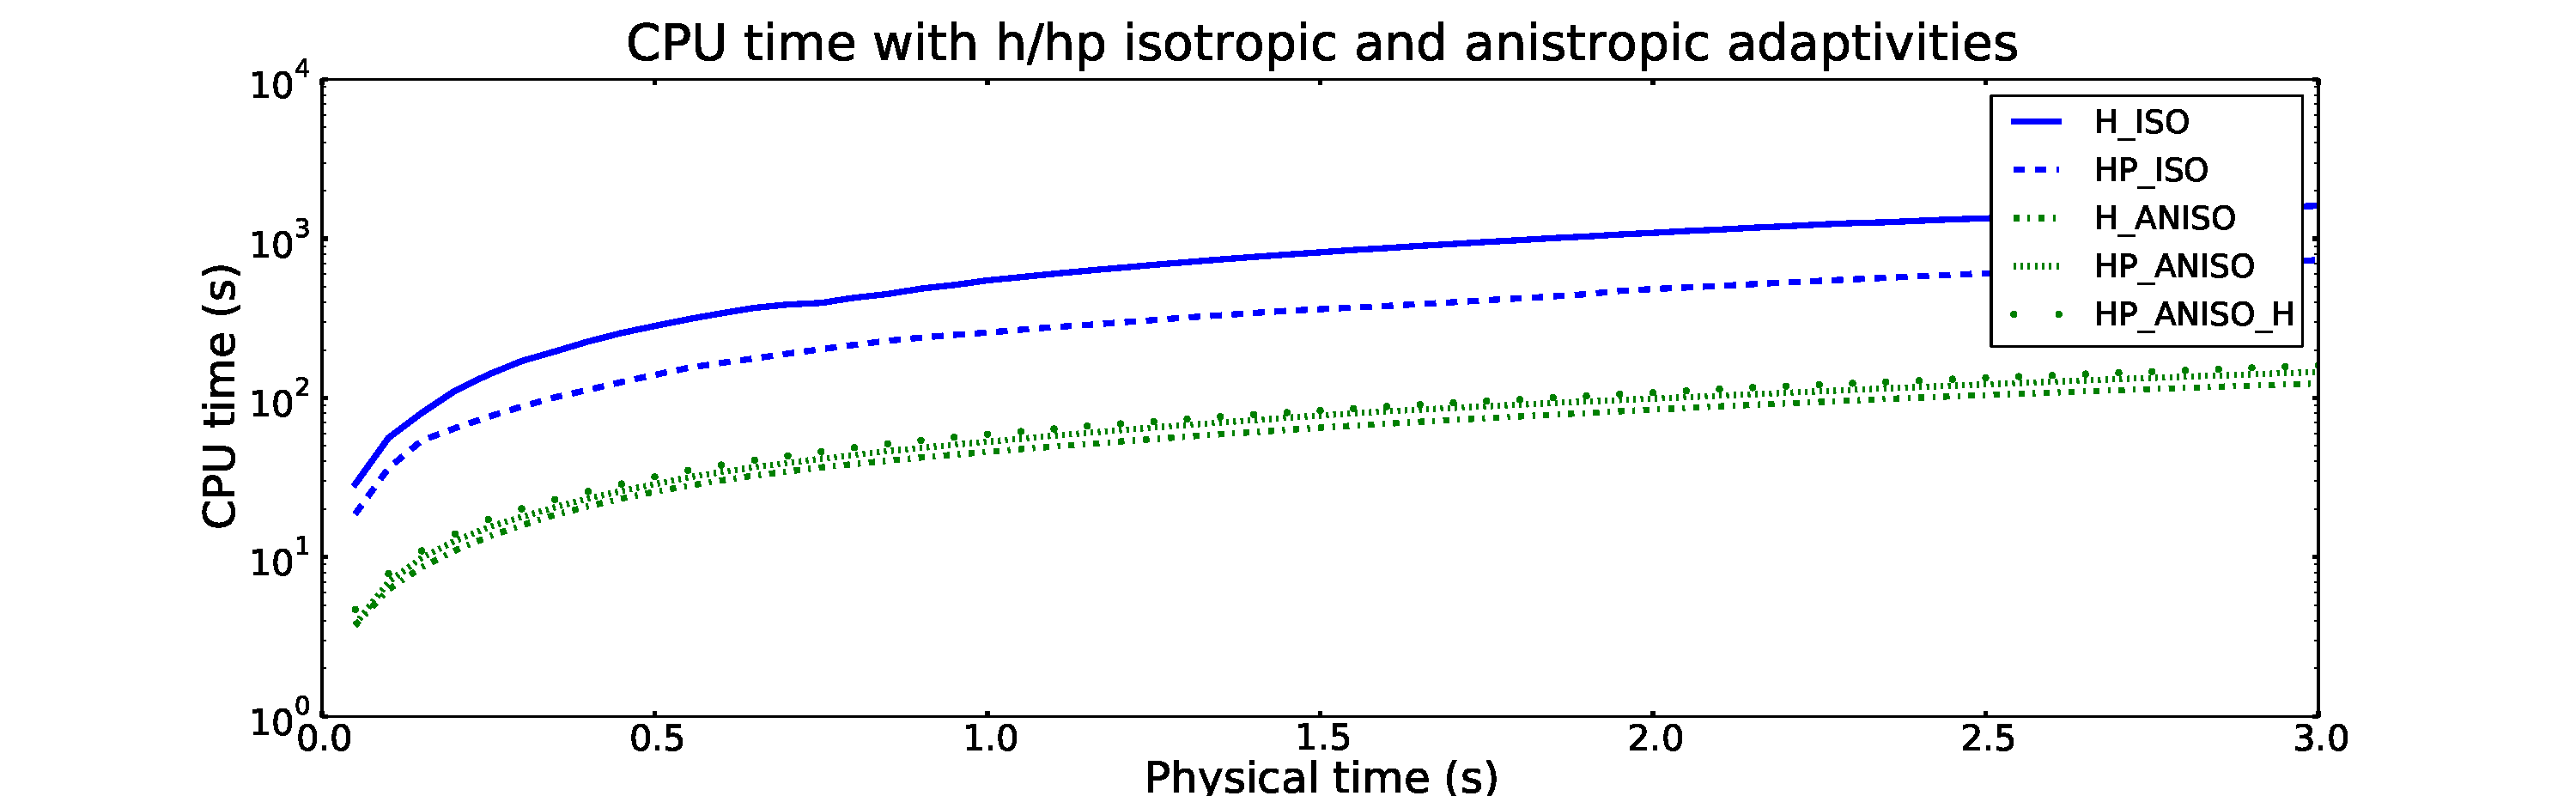
\includegraphics[width=\columnwidth]{isoaniso_cpu}
  \caption{\label{fig:isoanisocpu} Cumulative CPU time as a function of physical time 
  for multi-mesh configurations with H\_ISO, H\_ANISO,
  HP\_ISO, and HP\_ANISO adaptivity modes.}
  \end{centering}
\end{figure}

\noindent
Figs.~\ref{fig:isoanisopdof} and \ref{fig:isoanisopcpu} present a similar 
comparsion for the P\_ISO, P\_ANISO, and HP\_ANISO\_P modes. Recall that these 
computations use a different initial mesh that was a-priori refined in space.

\newpage

\begin{figure}[!ht]
  \begin{centering}
  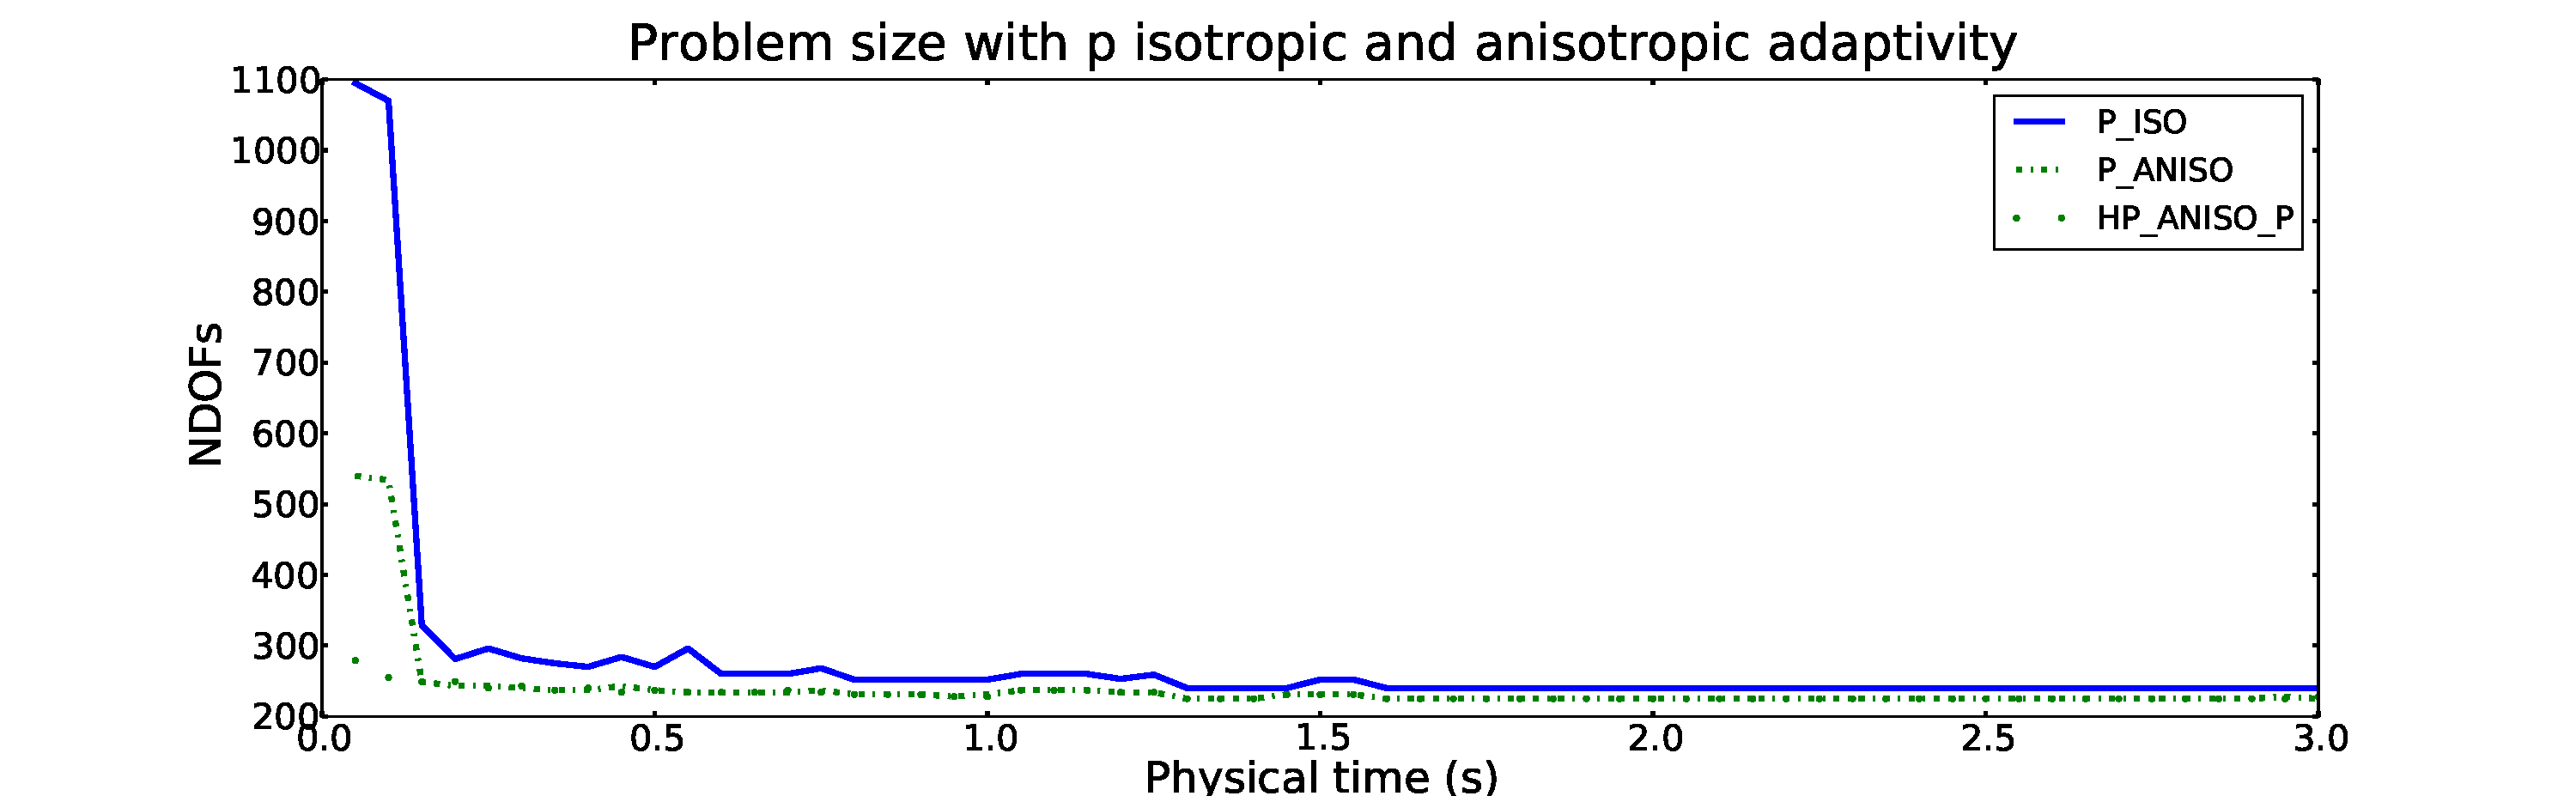
\includegraphics[width=\columnwidth]{isoanisop_dof}
  \caption{\label{fig:isoanisopdof} Number of DOF as a function of physical time
  for multi-mesh configurations with P\_ISO, P\_ANISO, and
  HP\_ANISO\_P adaptivity modes.}
  \end{centering}
\end{figure}

\begin{figure}[!ht]
  \begin{centering}
  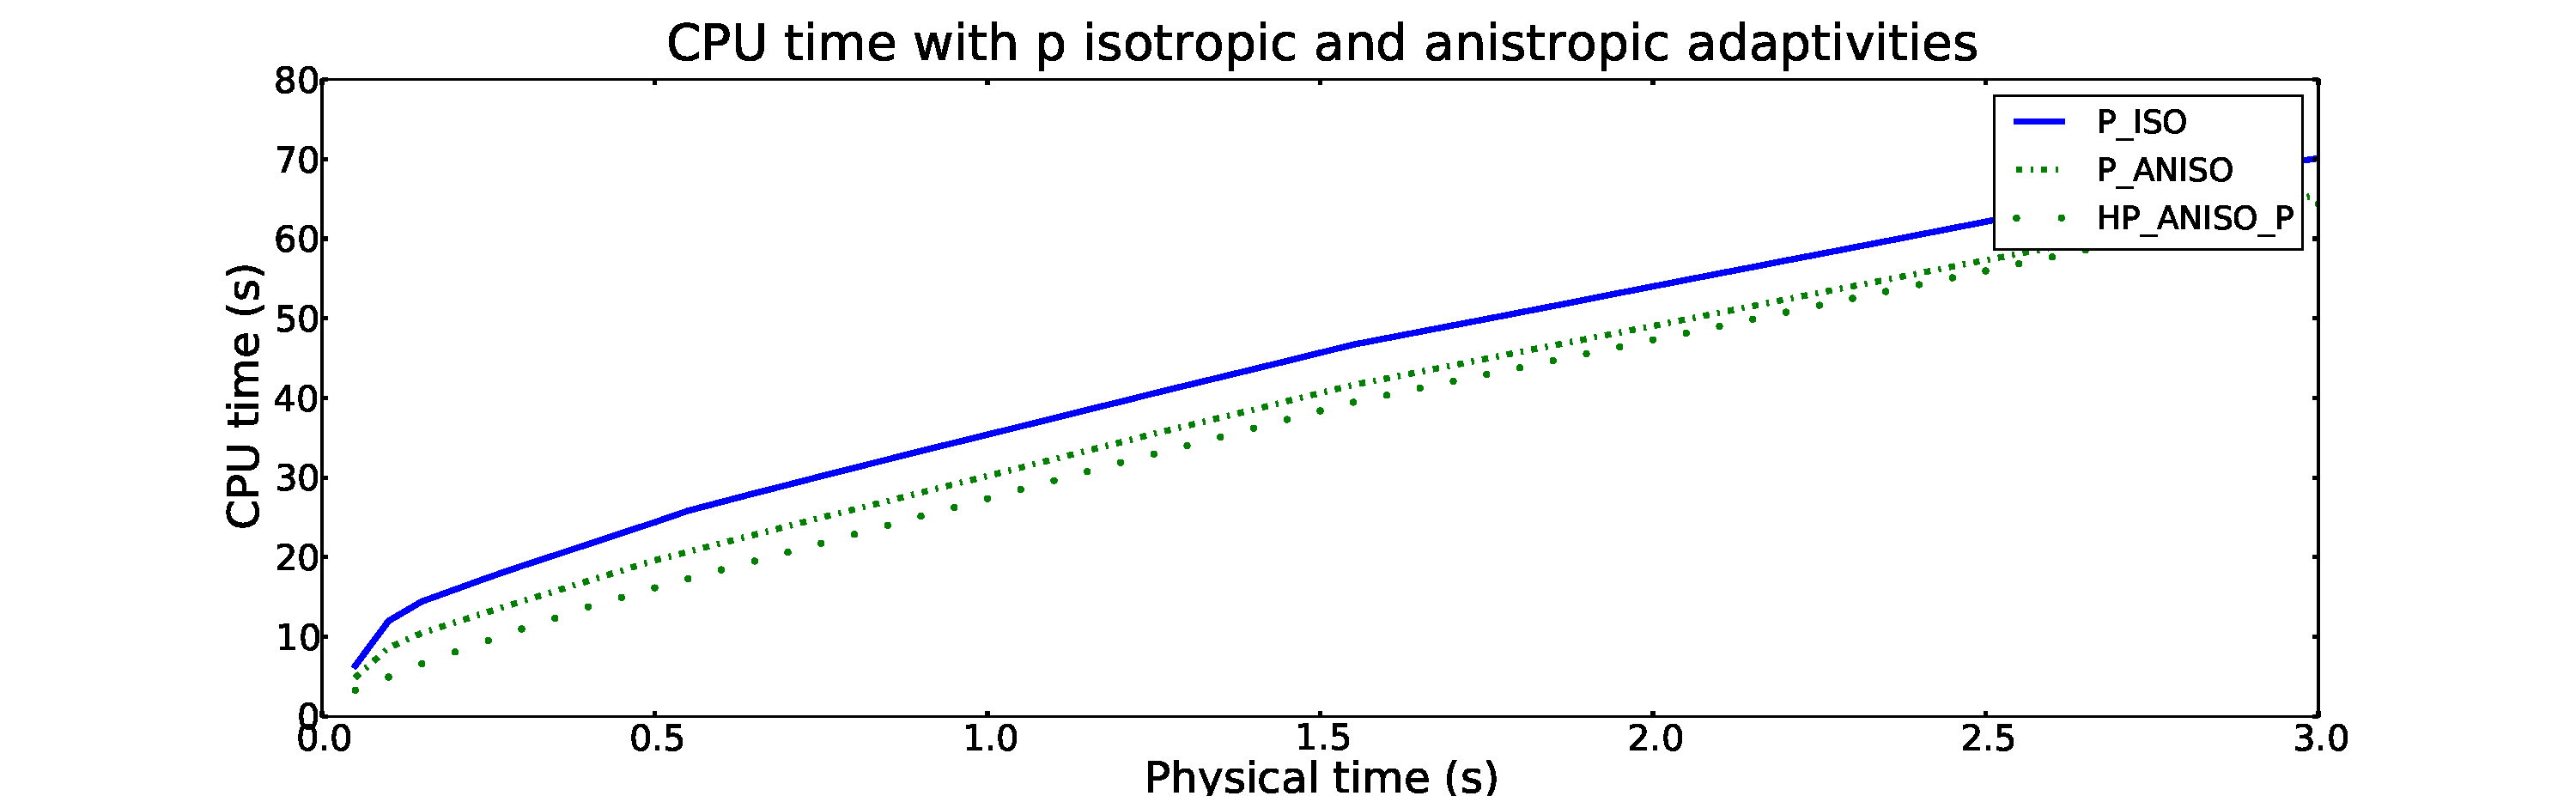
\includegraphics[width=\columnwidth]{isoanisop_cpu}
  \caption{\label{fig:isoanisopcpu} Cumulative CPU times as a function of physical time
  for multi-mesh configurations with P\_ISO, P\_ANISO, and
  HP\_ANISO\_P adaptivity modes.}
  \end{centering}
\end{figure}

As a conclusion, the reader can see that the anisotropic adaptivity modes always perform better than 
the isotropic ones. In particular, HP\_ANISO results into the smallest problem size. 
In the \emph{p}-adaptivity group, HP\_ANISO\_P leads to a small problem size
consistently in each time step, whereas P\_ISO and P\_ANISO yield large problems
during the first few time steps. 

%
%\subsection{Quantitative analysis of the refinement modes}
%
%Based on the results in the previous subsection, H\_ANISO, HP\_ANISO,
%and HP\_ANISO\_H from the \emph{hp/h}-adaptivity group and HP\_ANISO\_P
%from \emph{p}-adaptivity group will be compared
%in terms of NDOFs and cumulative CPU time. 
%In all of the cases, the relative 
%error at each time step remained below
%the threshold which was set to $e_{th}=0.5\%$ between the coarse mesh
%and fine mesh solutions, therefore the error-time plot will not be considered.
%
%\begin{figure}[!ht]
%  \begin{centering}
%  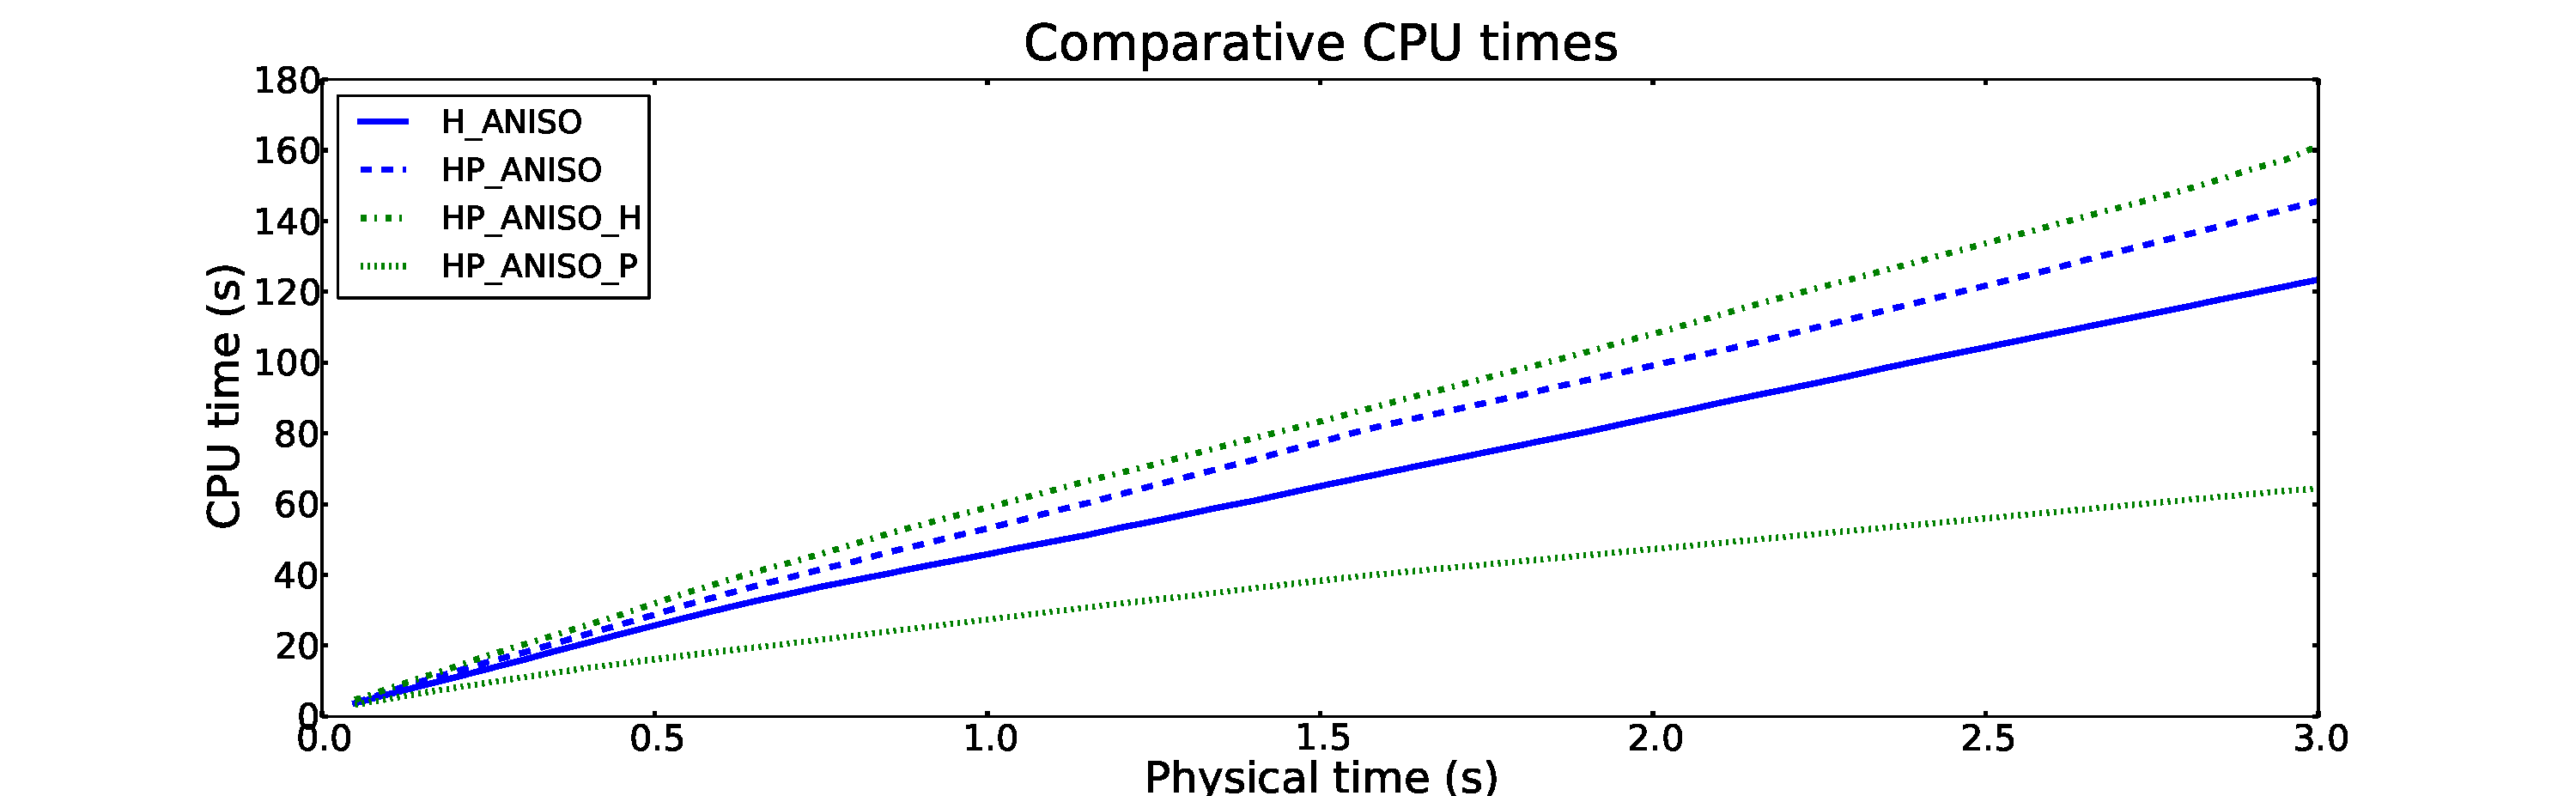
\includegraphics[width=\columnwidth]{cpu}
%  \caption{\label{fig:cpu} Comparative cumulative CPU time for different refinement modes.}
%  \end{centering}
%\end{figure}
%
%\begin{figure}[!ht]
%  \begin{centering}
%  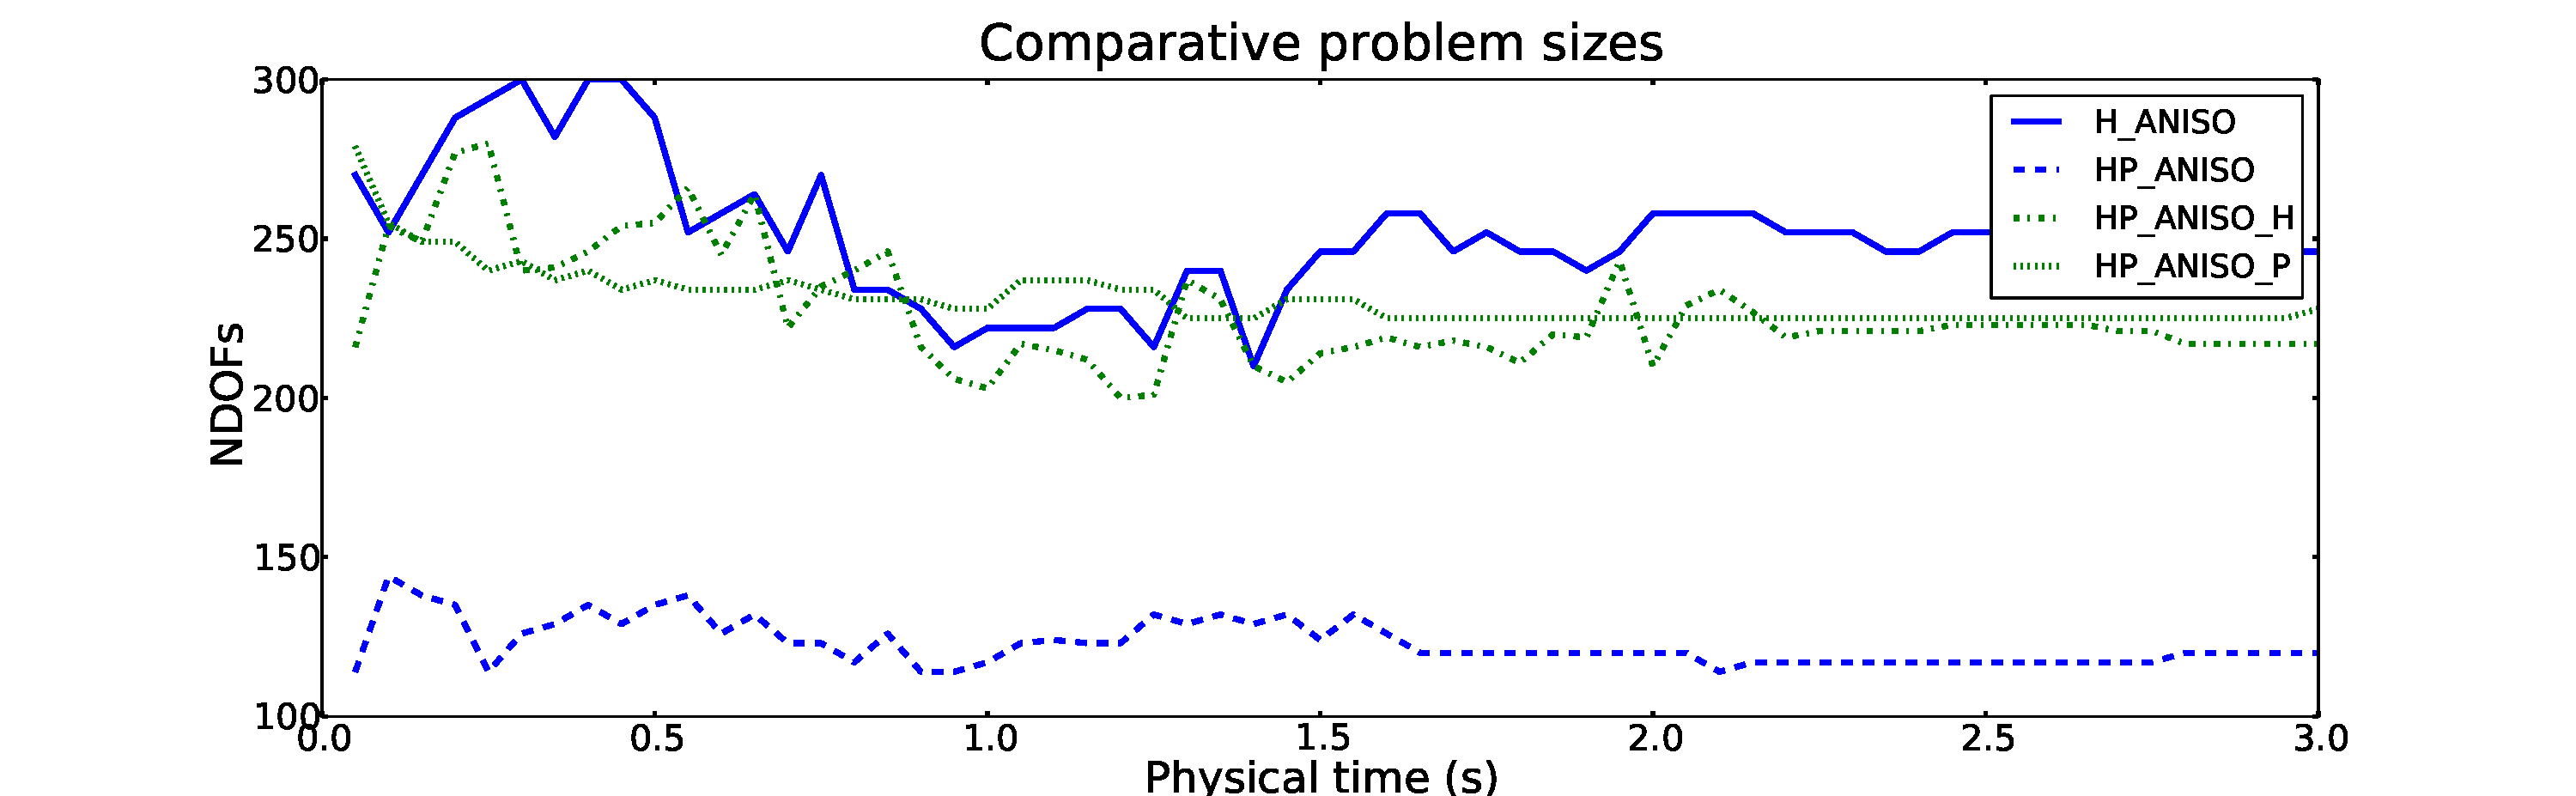
\includegraphics[width=\columnwidth]{dof}
%  \caption{\label{fig:dof} Comparative NDOFs at each time step for 
%  different refinement modes.}
%  \end{centering}
%\end{figure}
%
%Fig.~\ref{fig:cpu} shows the cumulative CPU time for different refinement 
%modes at each time step --- the results were recorded on the same computer
%for the CPU times to be comparable.
%We see that HP\_ANISO\_H and HP\_ANISO require the most
%resources. This can be understood from the fact that in case of these 
%refinement modes the adaptivity algorithm has the largest number of 
%candidates (see Section.~\ref{sec:model} and Fig.~\ref{fig:refinements})
%from which a particular refinement can be chosen.
%At the same time, HP\_ANISO\_P is the fastest compared to the other refinement modes.
%This can be attributed to the finer inital mesh.
%
%Fig.~\ref{fig:dof} shows the NDOFs at each time step.
%It can be seen that the HP\_ANISO results in the 
%smallest problem size --- $N_{DOF} \approx 125$. 
%All the other refinement modes result in a 
%problem size of approximately ($N_{DOF} \approx 250$). Therefore
%the HP\_ANISO is the most efficient in terms of memory consumption.
%
%As we have filtered out
%two notable refinement modes for the given problem --- HP\_ANISO\_P because of the fast
%calculation, and HP\_ANISO because of the small problem size. In the following
%subsection, some optimizations to reduce the CPU time of
%HP\_ANISO and reduce the NDOFs of HP\_ANISO\_P will be considered.


\subsection{Optimization of the HP\_ANISO and HP\_ANISO\_P adaptivity modes}

\begin{figure}[!ht]
  \begin{centering}
  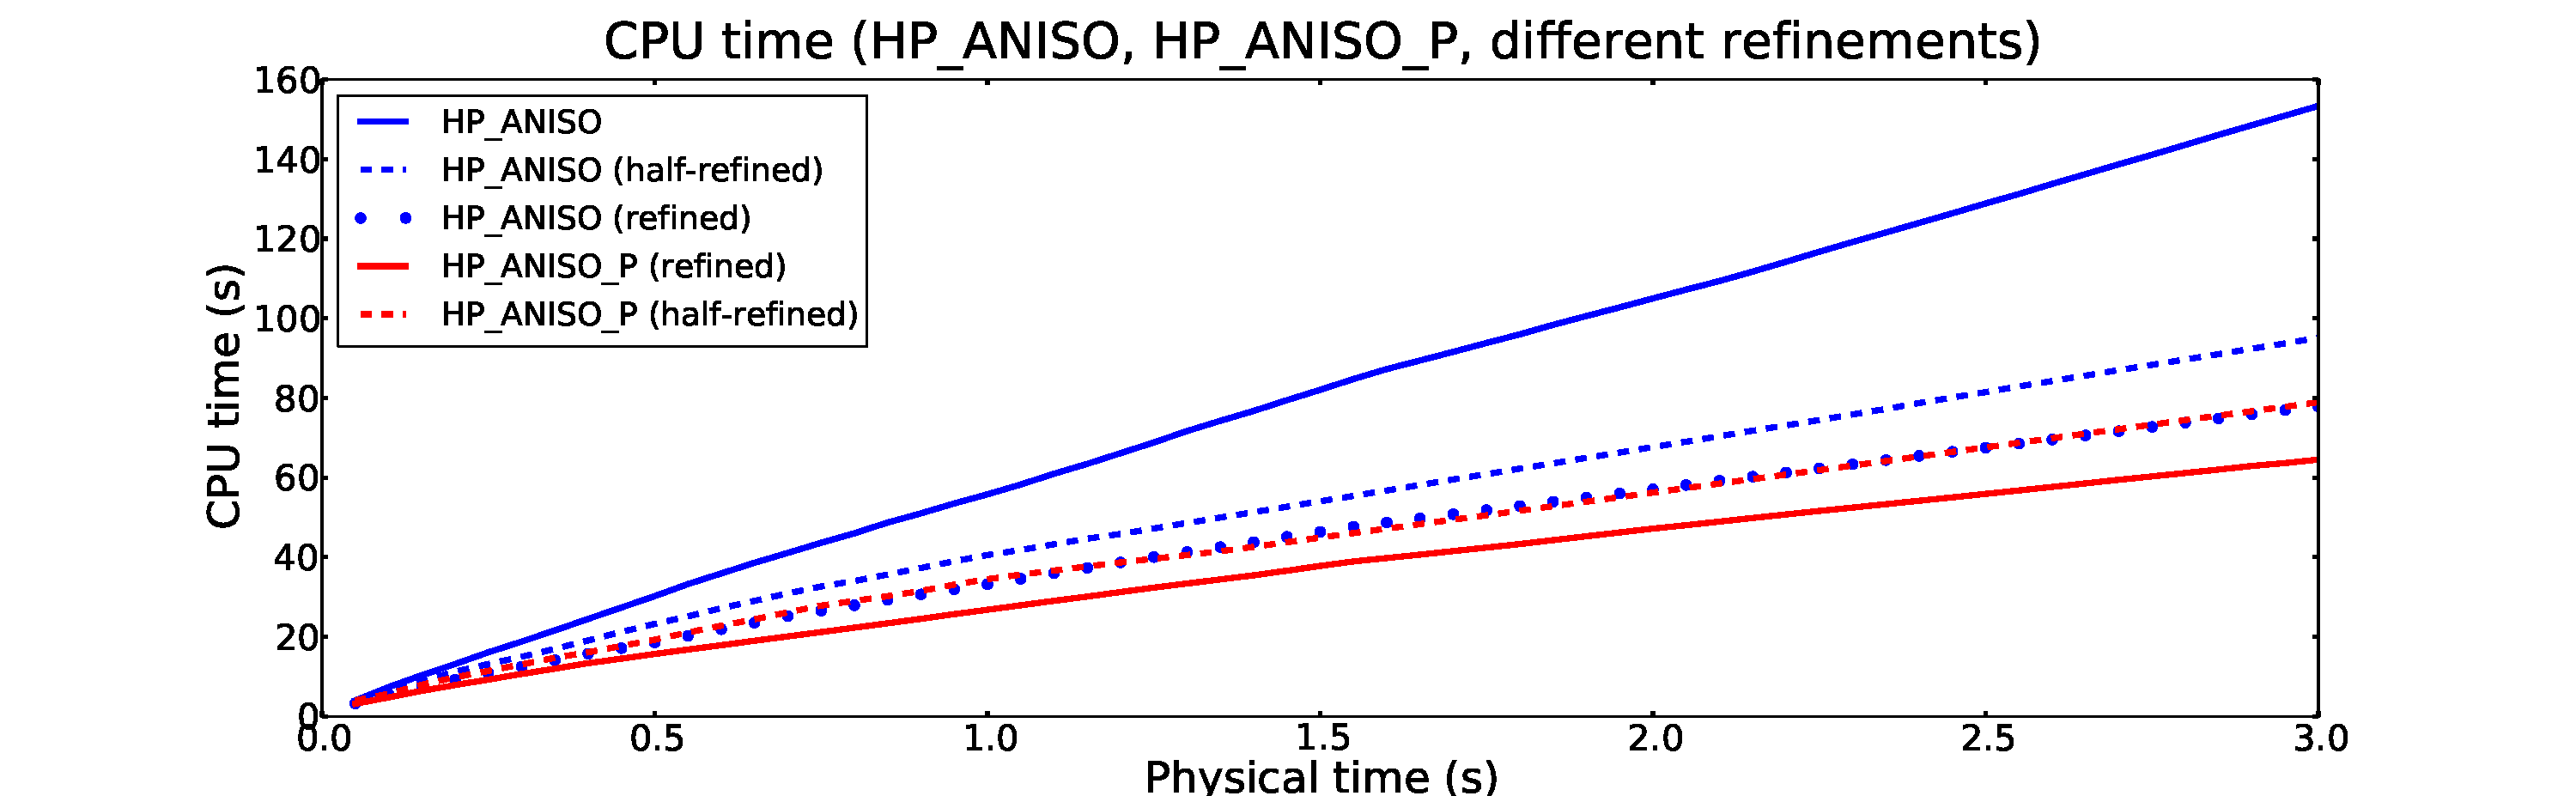
\includegraphics[width=\columnwidth]{refined_cpu}
  \caption{\label{fig:refined-cpu} Cumulative CPU time for HP\_ANISO and HP\_ANISO\_P
  with different initial meshes.}
  \end{centering}
\end{figure}

\begin{figure}[!ht]
  \begin{centering}
  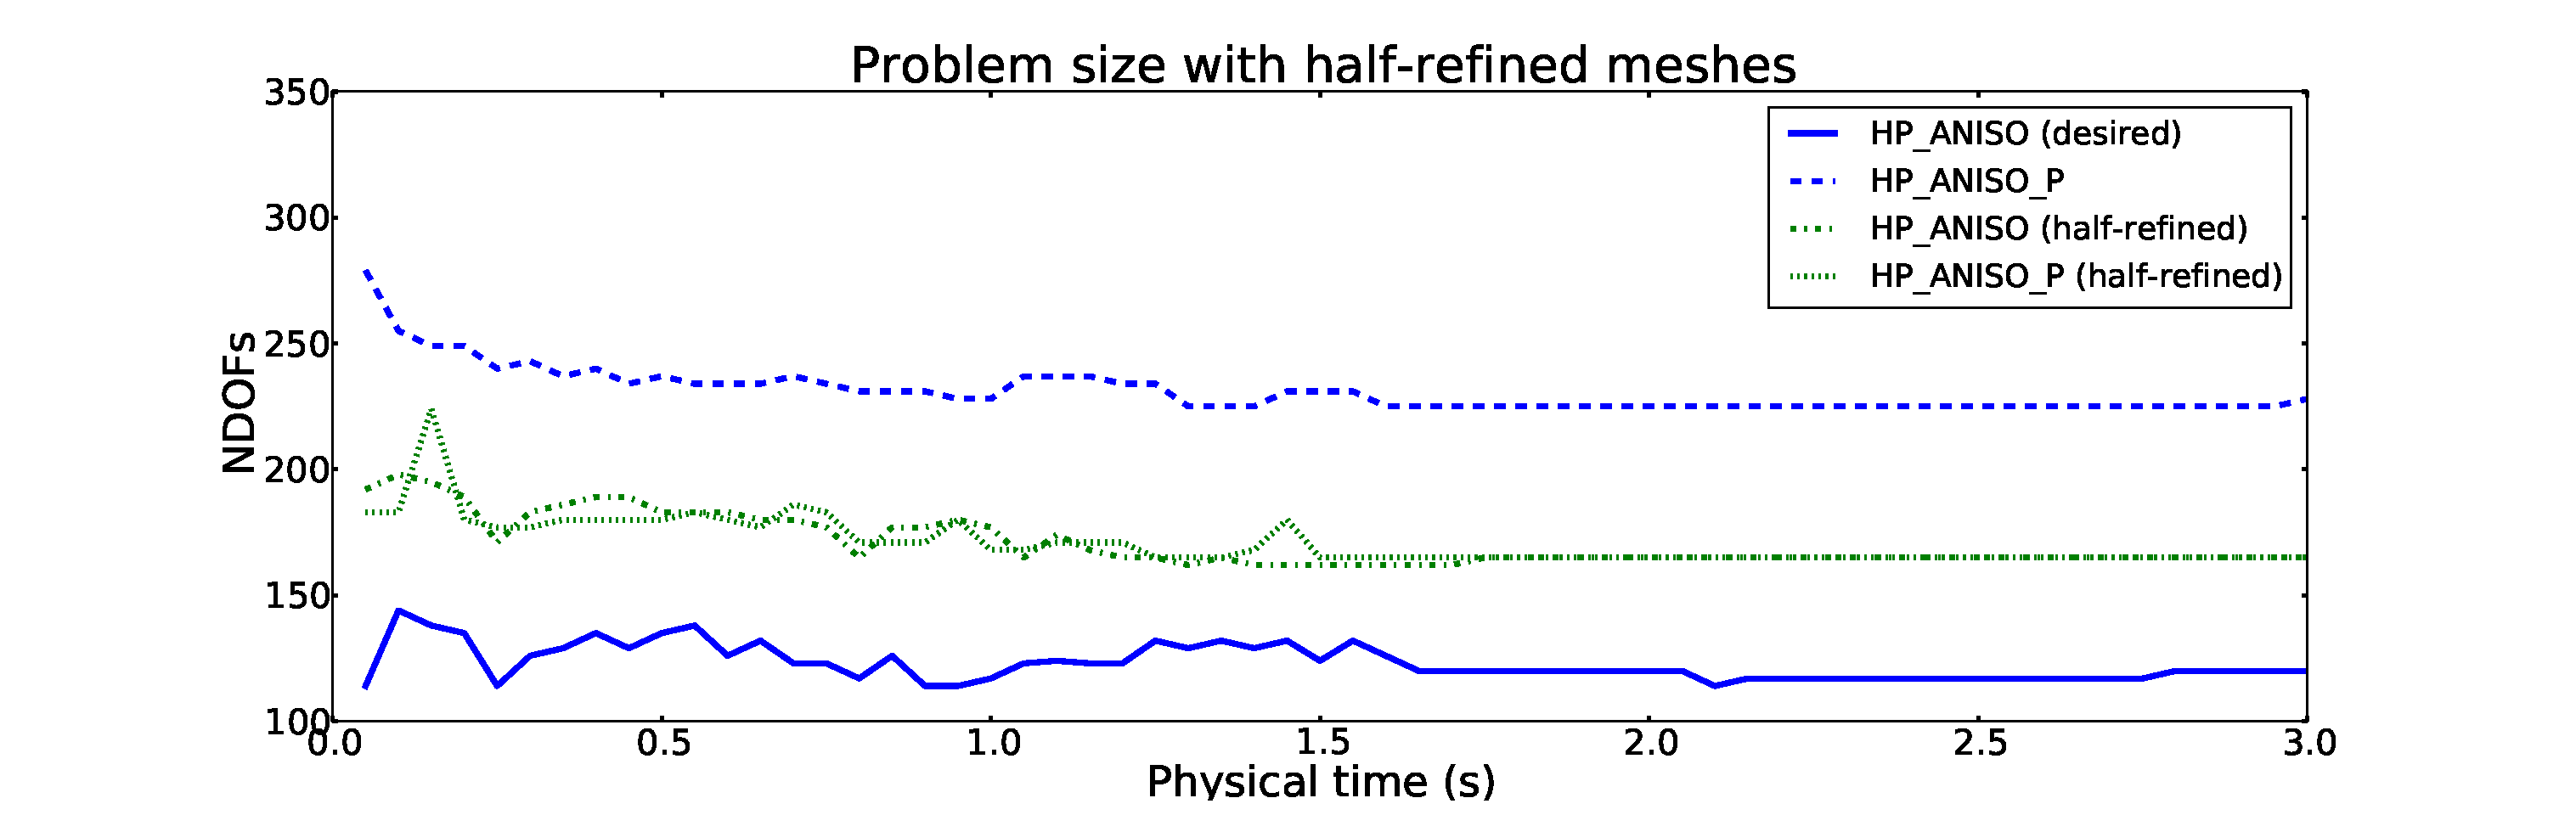
\includegraphics[width=\columnwidth]{refined_dof}
  \caption{\label{fig:refined-dof} NDOFs at each time step for
  HP\_ANISO and HP\_ANISO\_P with different meshes.}
  \end{centering}
\end{figure}

When it comes to a large domain or 3D modeling, the problem
size becomes a very important factor. Namely, 3D full scale solutions tend to use
a lot of memory. Therefore, we consider HP\_ANISO the most
suitable refinement mode for the given problem. 
Hence, some ways to optimize the HP\_ANISO model
to improve the CPU time factor without significantly 
compromising the NDOFs will be considered. 
The desirable output would be HP\_ANISO problem size
close to HP\_ANISO\_P CPU time. 
One way to optimize the problem
is to choose more refined initial mesh. Another way would be to change
the refinement frequency during the solving process. Theoretically it 
could result in a fewer adaptivity steps which are rather expensive in terms
of CPU time. Recall that up to this point,
the initial mesh was loaded in the beginning of each time step. 
True, by employing the optimizations, one must know something about the problem
and its solution beforehand. However, it could still be practial when solving a real problem
in a large domain.

The problem size and CPU time with HP\_ANISO
and HP\_ANISO\_P adaptivities on more refined initial mesh (see Fig.~\ref{fig:mesh}~(c))
compared to the coarse initial mesh (Fig.~\ref{fig:mesh}~(a)) and 
HP\_ANISO\_P solution are shown in Fig.~\ref{fig:refined-cpu} and Fig.~\ref{fig:refined-dof}.
By using initially more refined mesh, the problem solving time
can be reduced in case of HP\_ANISO, at the same time, the problem size increases
as the initial mesh is not necessarily the most optimal one.
However, in this situation, HP\_ANISO\_P and HP\_ANISO perform equally well.

\begin{figure}[!ht]
  \begin{centering}
  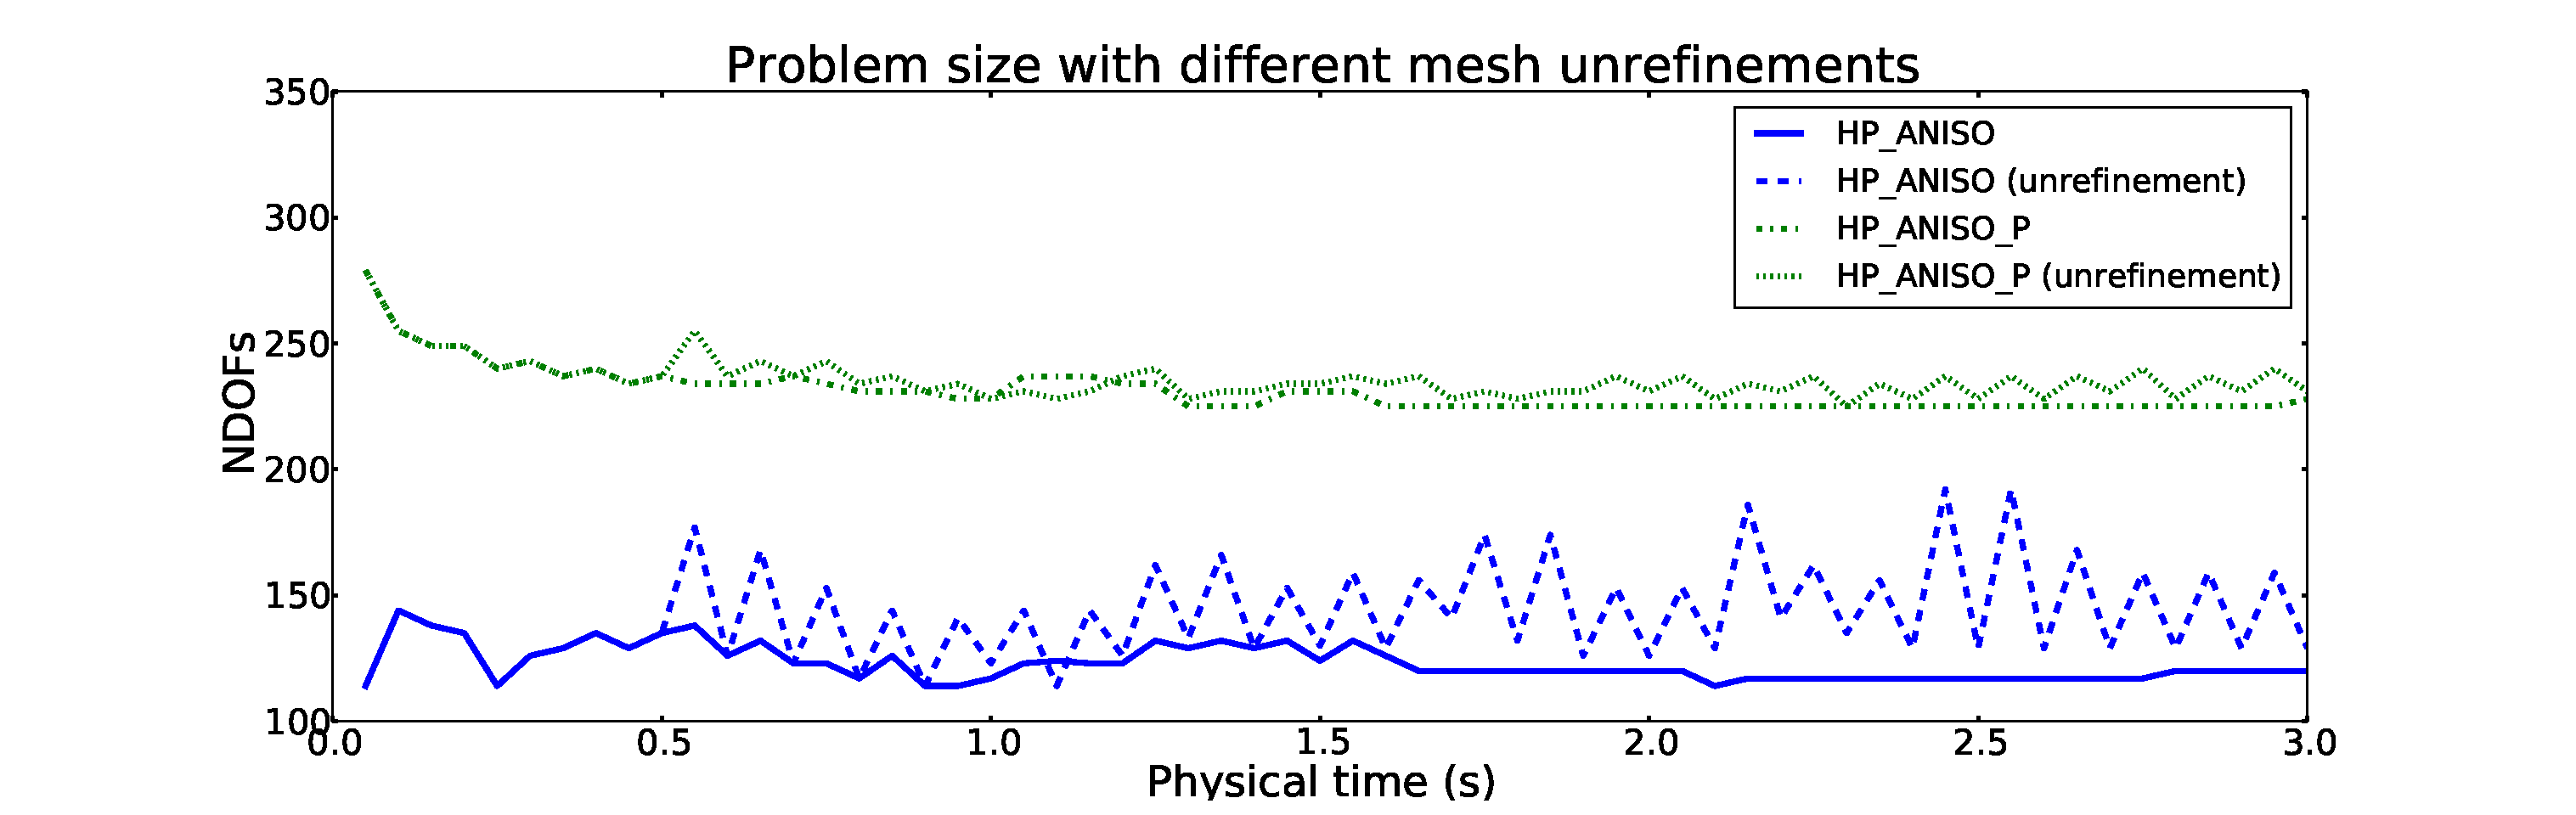
\includegraphics[width=\columnwidth]{unreffreq_dof}
  \caption{\label{fig:unreffreq-dof} NDOFs at each time step for
  HP\_ANISO and HP\_ANISO\_P with mesh unrefinement at each time step and at over each
  	time step after first $0.5\ s$ physical solution time.}
  \end{centering}
\end{figure}
The next proposed optimization involved changing the unrefinement frequency.
It is known that the concentration gradient $\nabla C$ changes the most in the initial phase
of the calculation, therefore, the unrefinement after each time step was performed
until $t=0.5\ s$ (physical time). After that, the
unrefinement was performed in $\Delta t = 0.10\ s$ interval.
However, this optimization does not appear to result in a stable solution, 
i.e. the problem size 
does not remain steady, but starts to oscillate depending on the unrefinement
frequency. This is shown in Fig.~\ref{fig:unreffreq-dof}. 

Therefore varying the unrefinement frequency will
likely not result in desired results in real applications for given system of equation.
At the same time, by varying the initial mesh size, optimal initial mesh could be found
for both HP\_ANISO and HP\_ANISO\_P refinement modes.
	 
\subsection{More general results}
\begin{figure}[!ht]
  \begin{centering}
  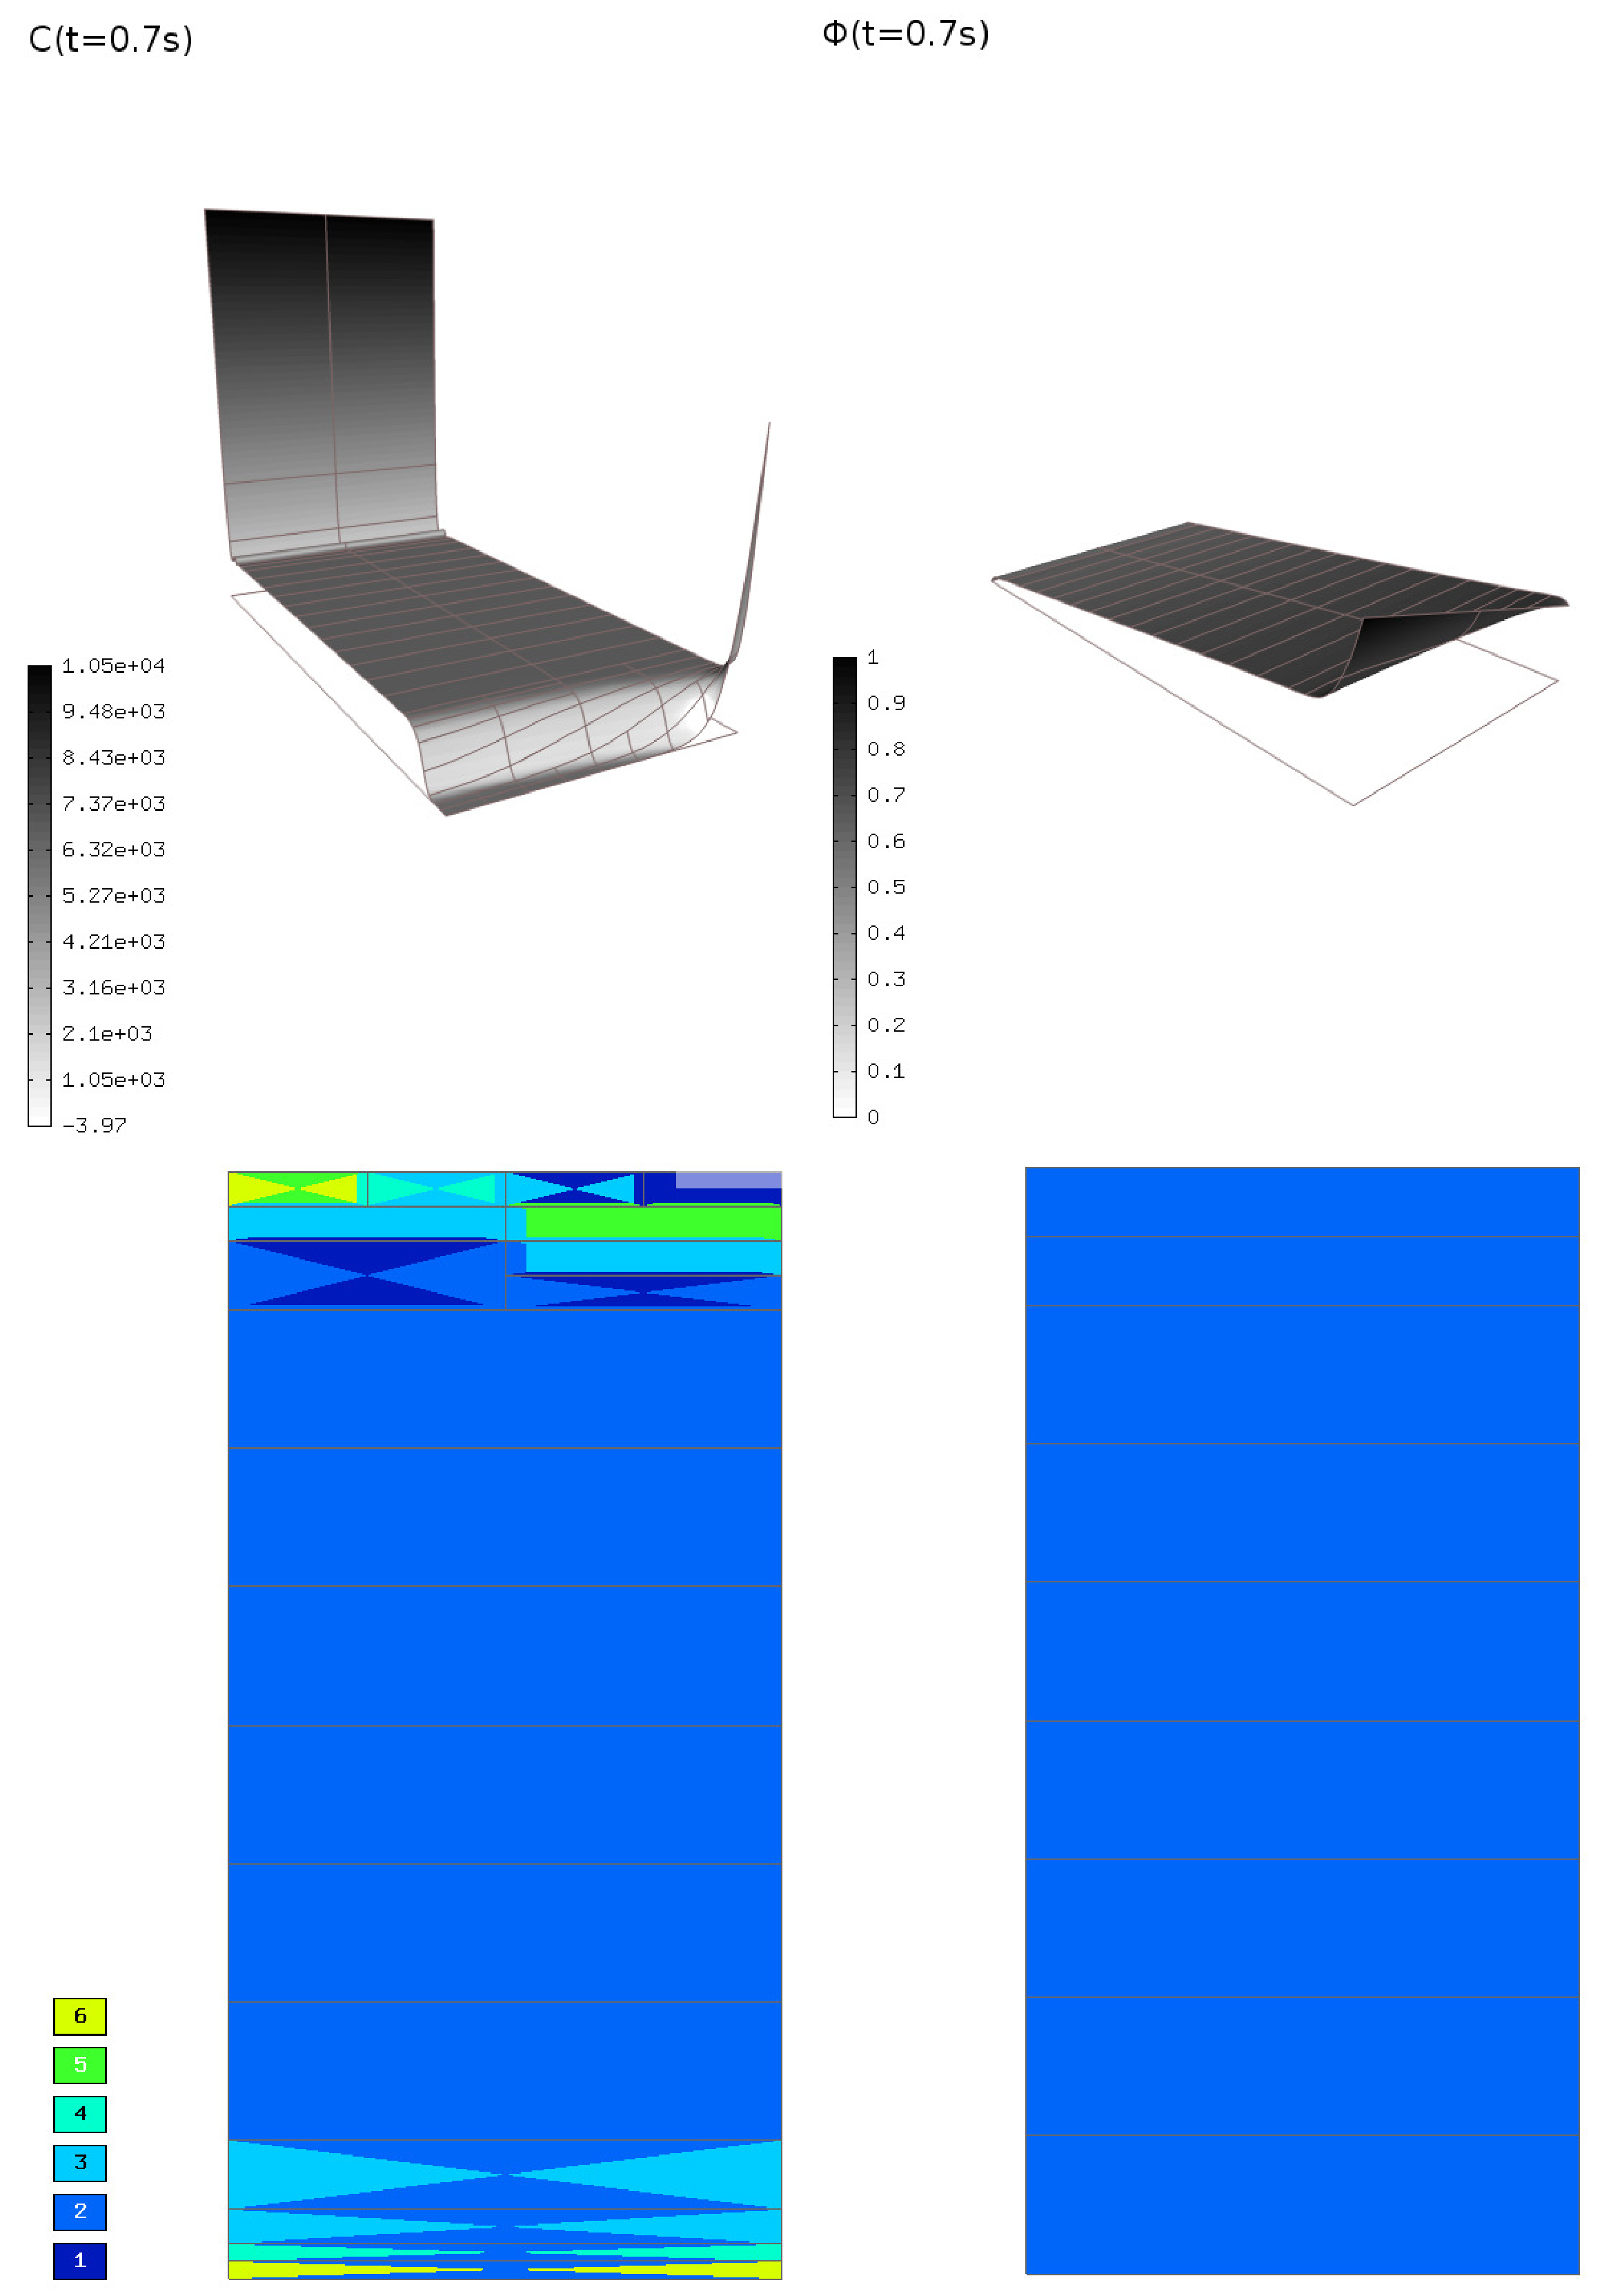
\includegraphics[width=.75\columnwidth]{cphiorders}
  \caption{\label{fig:cphi-orders} Solutions $C$ and $\phi$
  and corresponding polynomial degrees of the elements at
  $t=0.7\ s$. HP\_ANISO refinement mode was used. The height
  in the solution graphs indicates the value.}
  \end{centering}
\end{figure}

Based on the results, cation concentration and voltage was calculated
for different boundary conditions.
For instance, when voltage is applied as follows
\begin{equation}
  \phi_{\Omega_1}=0.5\frac{x}{width_{\Omega_1}}+0.5,
\end{equation}
the concentration gradient $\nabla C$ and the voltage gradient $\nabla \phi$ are no
longer effectively 1D.
The calculated $C$ and $\phi$ in $\Omega$ and corresponding meshes and polynomial
degrees of the elements are shown in Fig.~\ref{fig:cphi-orders}.
HP\_ANISO refinement mode was used. Notice that the solution
is different to the one in Fig.~\ref{fig:cphi} and the adapted mesh and the
polynomial degrees are also more complicated than in Fig.~\ref{fig:poly}.
It must be noted that in case of non uniform boundary conditions which
results in 2D problem, refined initial mesh was more efficient to use.
